\chapter{Visores web modificados}\label{cap.Visores}
En este capitulo se va a explicar como se han modificado los visores con tecnologías web existentes en la plataforma JdeRobot y desarrollados por Aitor Martínez en su TFG\footnote{\url{https://jderobot.org/Aitormf-tfg}}, para que utilicen el \textit{middleware} de comunicación ROS, además de ICE. Por otro lado, se le añadirá la posibilidad de ser ejecutados mediante el entorno Electron, además de en un navegador web. Estos tres visores son \texttt{CamVizWeb}, \texttt{TurtlebotVizWeb} y \texttt{DroneVizWeb}.

\section{CamVizWeb}
Se trata de un visor de imágenes desarrollado con tecnologías web, que usa los middleware de comunicación ICE y ROS  y pude ser ejecutados con Electron o en un navegador web.

\subsection{Diseño}
El visor previamente solo contaba con el \textit{middleware} ICE para realizar la comunicación, por lo que su funcionalidad estaba limitada a los drivers que son capaces de comunicarse de esta forma. Sin embargo, con esta extensión, se amplia el abanico de drivers que pueden conectarse al permitir la utilización tanto de ICE como de ROS. La figura 4.1 muestra el diagrama de bloques de su funcionamiento hasta ahora, mientras que la figura 4.2 muestra el diagrama de bloques tras habilitar la comunicación mediante las dos vías.

\begin{figure}[H]
  \begin{center}
    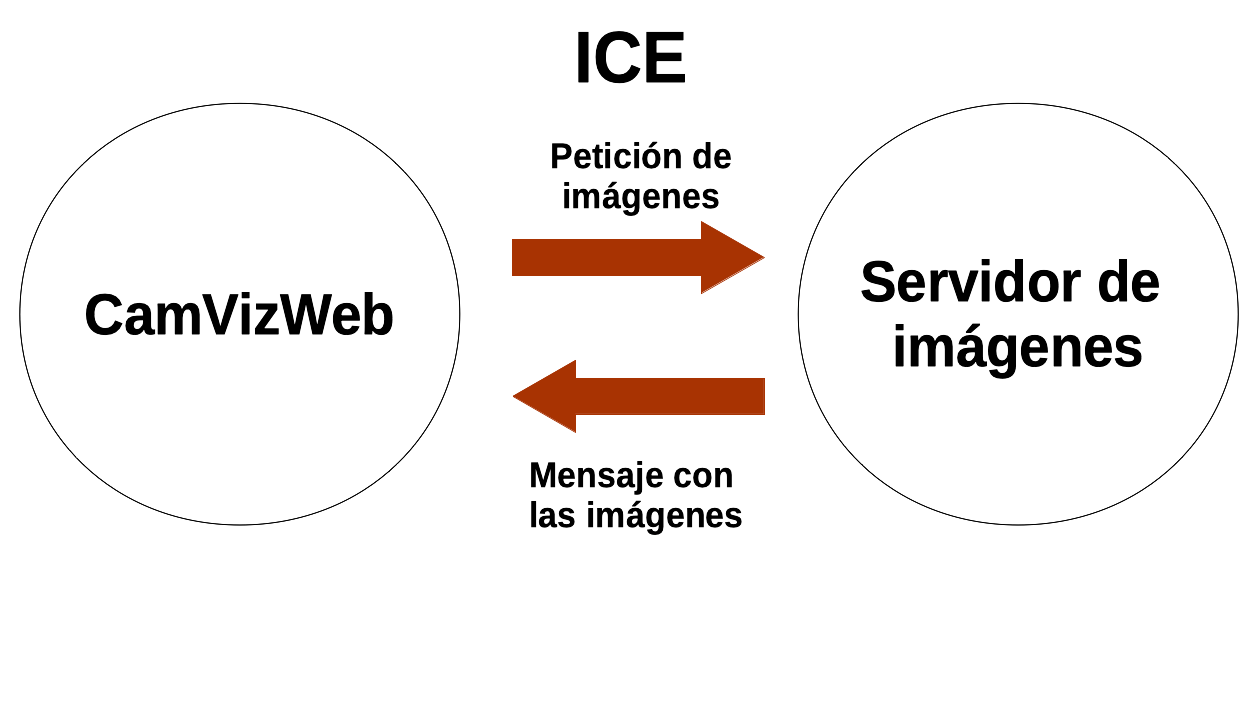
\includegraphics[width=0.8\textwidth]{figures/esquemacamviz1.png}
		\caption{Diagrama de bloques previo del sistema}
		\label{fig.esquemacamviz1}
		\end{center}
\end{figure}

\begin{figure}[H]
  \begin{center}
    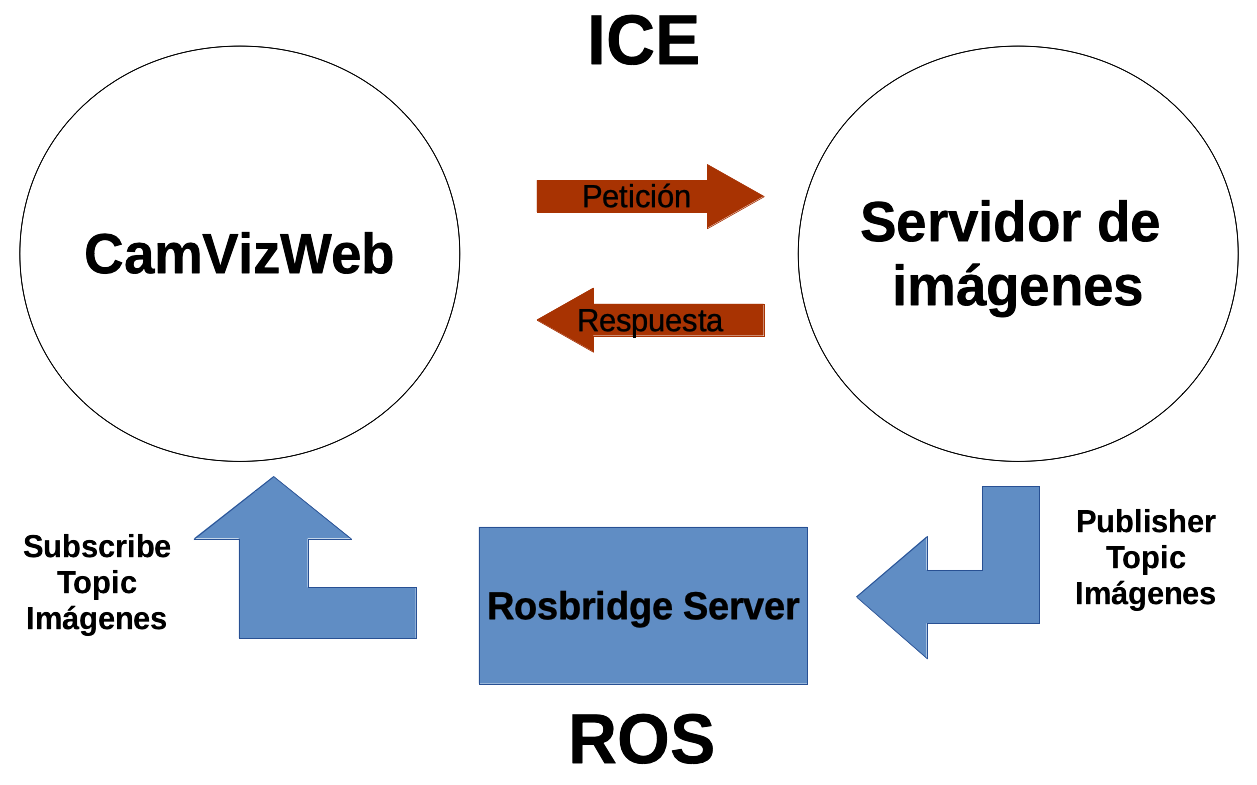
\includegraphics[width=0.8\textwidth]{figures/esquemacamviz2.png}
		\caption{Diagrama de bloques actual del sistema}
		\label{fig.esquemacamviz2}
		\end{center}
\end{figure}

En la figura 4.3 muestra la estructura del visor previo de una manera más detallada, mientras que la figura 4.4 muestra la estructura tras realizar la modificación.

\begin{figure}[H]
  \begin{center}
    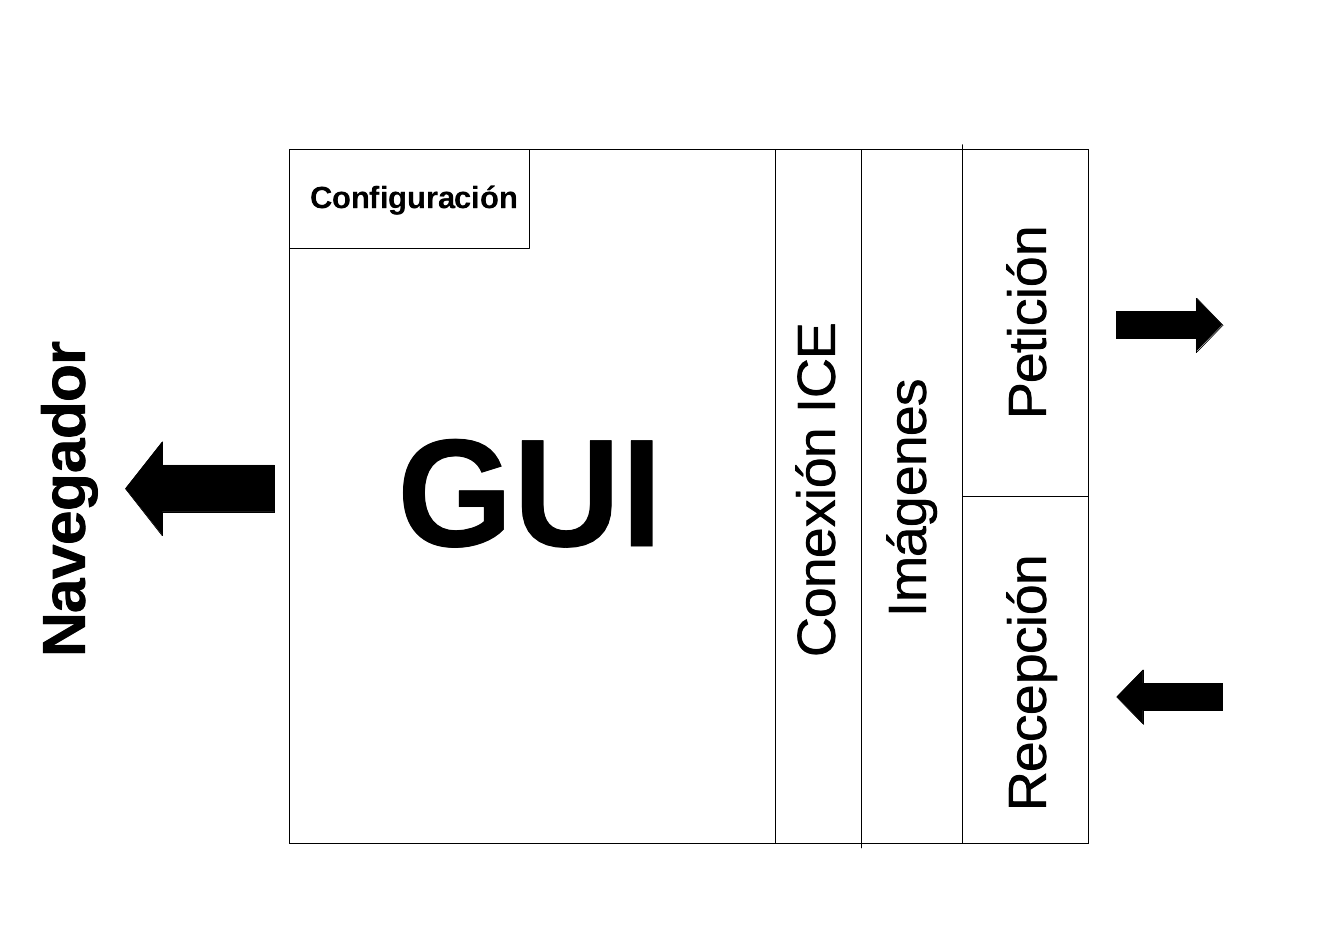
\includegraphics[width=0.8\textwidth]{figures/disenocamviz1.png}
		\caption{Estructura previa del visor}
		\label{fig.estructuracamviz2}
		\end{center}
\end{figure}

\begin{figure}[H]
  \begin{center}
    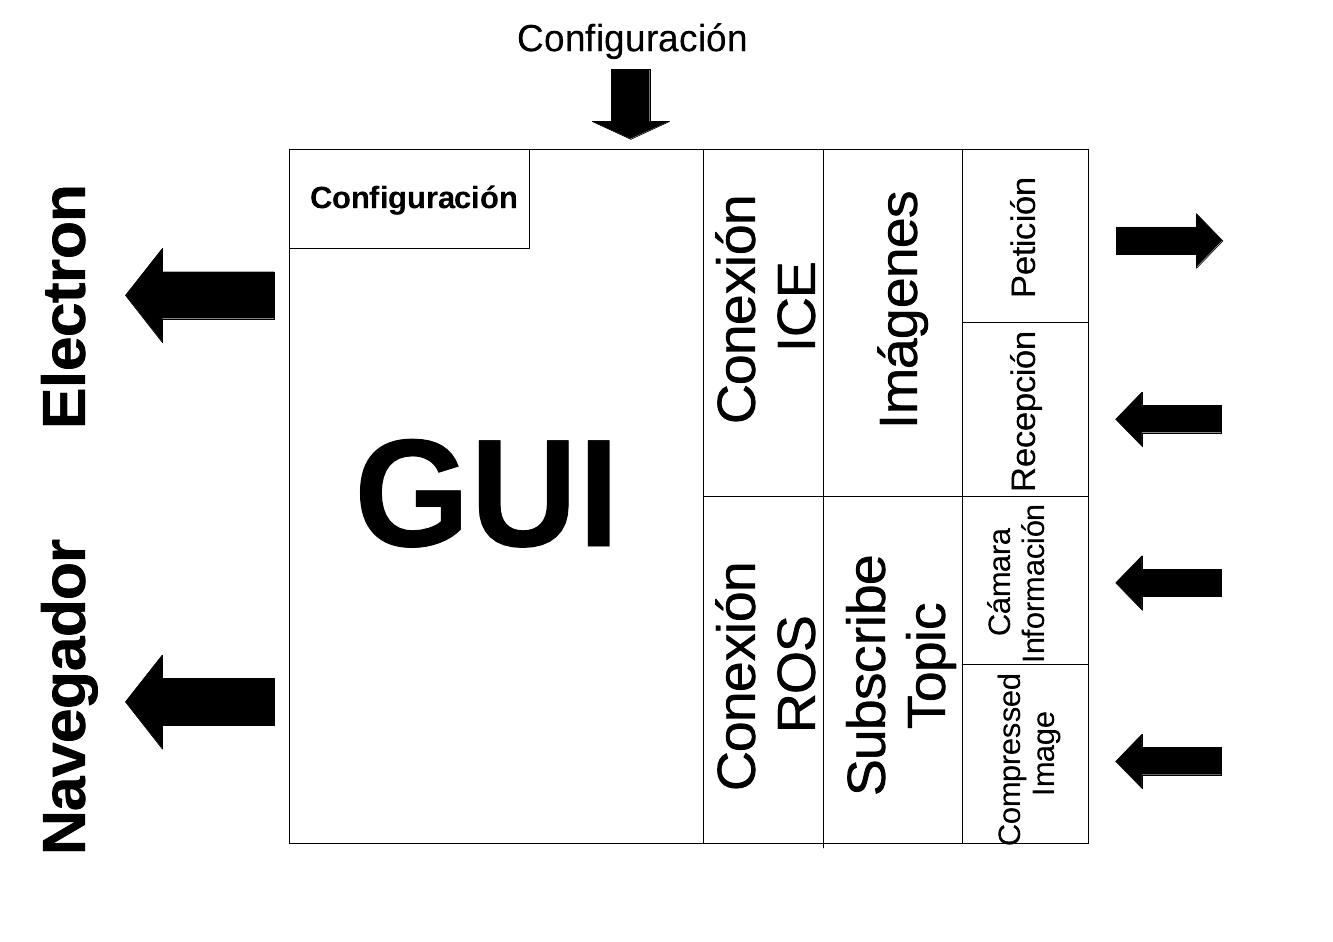
\includegraphics[width=0.8\textwidth]{figures/Camviz2.png}
		\caption{Estructura actual del visor}
		\label{fig.estructuracamviz2}
		\end{center}
\end{figure}

El visor esta dividido en dos partes: la interfaz gráfica y las conexiones. La interfaz gráfica contiene los elementos necesarios para visualizar las imágenes recibidas, además de contener un menu para realizar la configuración en tiempo de ejecución del visor.

Las conexiones están formadas a su vez por otras dos partes. La primera parte corresponde a la conexión mediante ICE para realizar las peticiones y recibir las imágenes, siendo esta comunicación la existente en el visor, por lo que no se va a profundizar en su funcionamiento. La segunda parte corresponde a la conexión con ROS y se obtienen los mensajes mediante los \textit{Subscribe} de ROS. Para obtener la misma información que se obtiene utilizando ICE, es necesario realizar dos \textit{Subscribe}. El primero se utiliza para obtener las imágenes mediante el tipo de mensaje de ROS \texttt{CompressedImage}, el segundo es el encargado de suministrar la información de la cámara (anchura, altura, etc) utilizando el mensaje de ROS \texttt{CameraInfo}.

Por otro lado, como se puede ver en la diferencia entre las figuras 4.3 y 4.4, el visor tiene dos novedades más. La primera corresponde al modo de ejecutarlo, ya que puede utilizarse Electron o un navegador web, esto proporciona al visor de ser ejecutado como una aplicación de escritorio haciendo del visor multiplataforma y sin el problema de compatibilidad entre navegadores. La otra novedad es la posibilidad de realizar la configuración previa al arranque del visor, utilizando para ello un fichero de formato \texttt{YAML}.

\subsection{Interfaz gráfica}
La interfaz gráfica se ha mantenido la existente previamente realizando las modificaciones necesarias para realizar la conexión mediante el middleware ROS. Esta interfaz esta formada por un elemento \texttt{Canvas} de HTML5, donde se mostrarán las imágenes, un cuadro donde irá la información acerca de la cámara y tres botones. El primer botón corresponde al botón de \textit{Start} para comenzar la recepción y visualización de imágenes, el segundo botón corresponde al botón de \textit{Stop} para parar la recepción y visualización, y el tercer botón corresponde al menú de configuración que al pulsarlo abrirá una ventana emergente.

\begin{figure}[H]
  \begin{center}
    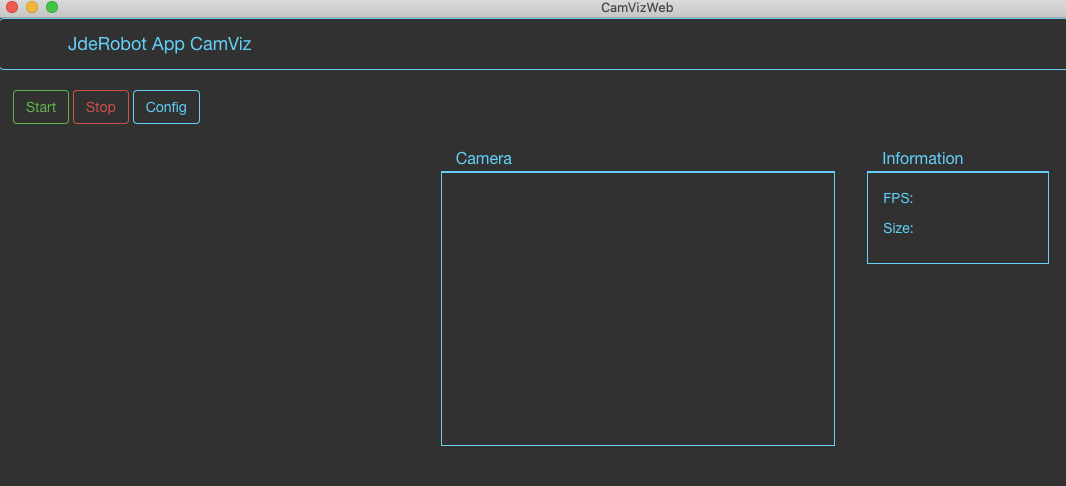
\includegraphics[width=0.8\textwidth]{figures/interfazcamviz.png}
		\caption{Interfaz gráfica del visor}
		\label{fig.iterfazcamviz}
		\end{center}
\end{figure}

Esta modificación se ha realizado sobre el menú de configuración para que cuando se abra la ventana emergente, se pueda seleccionar ROS o ICE. Para lograr esto, se ha añadido al archivo \texttt{index.html}un formulario de HTML que contiene dos botones, uno para ICE y otro para ROS. En el cuadro 4.1 se muestra el código añadido a este archivo.

\begin{lstlisting}[caption= Formulario para añadir al menu de configuración la posibilidad de conectarse mediante ICE o ROS, label=cod.formulariocamviz]
<form class="form-inline">
           <button id="DfIce" type="button">Ice</button>
           <button id="DfRos" type="button">Ros</button>
</form>
\end{lstlisting}

En la figura 4.5 se muestra como queda este menú tras añadir este formulario.

\begin{figure}[H]
  \begin{center}
    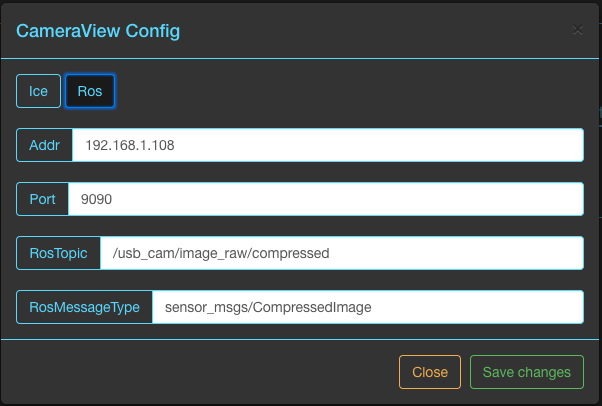
\includegraphics[width=0.8\textwidth]{figures/configuracioncamviz.png}
		\caption{Menu de configuración del visor}
		\label{fig.configuracioncamviz}
		\end{center}
\end{figure}

\subsection{Conexiones}

Como se ha indicado anteriormente el visor aceptaba conexiones únicamente mediante ICE, por lo que se modifica para que acepte también conexiones con ROS. En esta subsección se explica como se ha añadido la comunicación mediante el \textit{middleware} ROS.

\subsubsection{Establecimiento de la conexión}

La conexión se realiza utilizadno la biblioteca roslibjs que proporciona todo lo necesario. En el cuadro 4.2 se muestra como se realiza la conexión.

\begin{lstlisting}[caption= Establecimiento de la conexión ROS, label=cod.conexioncamviz]
var ros = new ROSLIB.Ros({
            url : "ws://IP:Puerto"
         });

ros.on('connection', function() {
             console.log("Connect websocket")
         });
ros.on('error', function(error) {
            console.log("Error to connect websocket")
});
\end{lstlisting}

Lo primero que se hace es definir la conexión mediante el objeto \texttt{ROSLIB.Ros} e indicando que se va a realizar mediante WebSockets y definiendo la IP y puerto de escucha el servidor intermedio Rosbridge Server. Creado este objeto, se establece la conexión con el servidor intermedio, llamando al método \texttt{ros.on} y pasando por parámetro el \textit{string} ``Connect'' y la función que se desea que se ejecute cuando se establezca la conexión. Si durante la fase de conexión ocurre algún error, se invocará al mismo método \texttt{ros.on}, pero en esta ocasión pasando por parámetro el \textit{string} ``error'' y la función que se ejecutará en caso de error.

\subsubsection{Estructura de los mensajes}
Como se ha indicado en la sección 4.1.1, se necesitan dos mensajes para obtener la misma información que se obtiene mediante ICE. Para ello, se definen dos mensajes de los tipos predeterminados de ROS y definidos en su documentación\footnote{\url{http://wiki.ros.org/common_msgs}}.

El mensaje con el que se recibirán las imágenes es del tipo \texttt{sensor\_msgs/CompressedImage}, que son imágenes comprimidas en formato jpeg. El motivo de esta elección es por la fácil compatibilidad entre este formato y los elementos \texttt{Canvas} de HTML5, lo que permite la visualización directa de las imágenes reduciendo al mínimo el retardo. Sin embargo, este tipo de mensaje no contiene información acerca de las propiedades de la cámara, por este motivo es necesario complementar este mensaje con otro.

El mensaje para recibir las propiedades de la cámara es del tipo \texttt{sensor\_msgs/CameraInfo}. Este mensaje da la información de la anchura y altura de cada imagen.

En el código del cuadro 4.3 muestra como se definen estos mensajes. En ambos casos se utiliza el objeto de roslibjs \texttt{ROSLIB.Topic}, indicándole la conexión ROS establecida anteriormente, el nombre del \textit{Topic}, que para el caso del mensaje con las imágenes se establecerá a través de la configuración del visor y para el caso de la información de la cámara será predeterminado, y el formato del mensaje, que son los indicados anteriormente para cada caso.

\begin{lstlisting}[caption= Definición de los mensajes ROS, label=cod.mensajescamviz]
var roscam = new ROSLIB.Topic({
            ros : ros,
            name : conf.topic,
            messageType : "sensor_msgs/CompressedImage"
});

var rosdescrip = new ROSLIB.Topic({
          ros: ros,
          name : "/usb_cam/camera_info",
          messageType: "sensor_msgs/CameraInfo"
})
\end{lstlisting}

\subsubsection{Subscripción a los \textit{Topic} y visualización de las imágenes}

Una vez que se han definido los mensajes, es hora de subscribirse a los \textit{Topic} para recibir los mensajes. Para realizar esto se ha definido la función \texttt{startStreaming} que se muestra en el cuadro 4.4.

\begin{lstlisting}[caption= Subscripción y visualización de las imágenes, label=cod.subscribecamviz]
var startStreaming = function(){
        var canvas = document.getElementById("camView");
        var fps = document.getElementById('fpsid');
        var size = document.getElementById(('sizeid');
        var ctx = canvas.getContext("2d");
        var imagedata = new Image();
        
        rosdescrip.subscribe(function(message){
          size.html(message.width + "x" + message.height);
        })
        
        roscam.subscribe(function(message){
        		if (message.format != null){
            		imagedata.src = "data:image/jpg;base64," + message.data;
            		imagedata.onload = function(){
              		ctx.drawImage(imagedata,0,0,canvas.width,canvas.height);
            	}
          	} else {
            		console.log(message);
          	}
          	var fps_2 = calculateFPS();
          	if (fps_2){
             		fps.html(Math.floor(fps_2));
          	}
      	});
}
\end{lstlisting}

Lo primero que se hace es establecer los elementos HTML dónde se va a mostrar los datos recibidos. Estos elementos son el canvas y el cuadro donde va la información acerca de las propiedades de la cámara y los fotogramas por segundo, siendo \texttt{fps} el elemento que contendrá la información sobre los fotogramas por segundo, y \texttt{size}, el elemento que contendrá la información sobre el tamaño de cada fotograma. Posteriormente se da el contexto al elemento \texttt{Canvas}  y se define la imagen que se va a mostrar como un objeto del tipo \texttt{Image}.

Una vez realizadas estas tareas previas, se realiza la subscripción a los \textit{Topics} indicados anteriormente. Se utiliza el método de roslibjs \texttt{subscrebe} pasando por parámetro la función con el código que se desea ejecutar una vez recibido los datos. Primero se subscribe a la información de la cámara y los datos recibidos se indica que se deben mostrar en el elemento HTML donde se muestra el tamaño de cada fotograma.
La segunda subscripción es la realizada para recibir las imágenes. Al mensaje recibido, se le añade el encabezado para indicar que se trata de imágenes comprimidas del tipo jpeg y posteriormente mediante el método \texttt{drawImage} que proporciona el elemento \texttt{Canvas}, se muestra las imágenes recibidas en este elemento pasando por parámetros la imagen con el encabezado y el tamaño del elemento \texttt{Canvas} .

Finalmente se calcula los fotogramas por segundo que se reciben, para ello se ha creado el método \texttt{calculateFPS()}, este método lo único que hace es restar a la marca de tiempo en la que se recibe el mensaje actual, la marca de tiempo del anterior mensaje recibido. El resultado de esta función se muestra en el elemento \texttt{fps}.

\subsection{Configuración}
El visor puede ser configurado por dos vías: mediante un fichero de configuración externo para configurar antes de arrancar o a través del menú de configuración de la interfaz gráfica para configurar en tiempo de ejecución.

Para la primera vía se ha decidido usar un archivo externo con formato ``YAML'' que es leído y su información cargada por el visor al arrancar. ``YAML'' es un formato de serialización de datos muy sencillo de usar y de leer por una aplicación. Usando una única línea de código, se puede cargar y guardar en una variable la información que contiene un archivo de este tipo. El código del cuadro 4.5 muestra como realizar la lectura del fichero.
\begin{lstlisting}[caption = Leer el fichero ``YAML'' con la configuración y guardar la información en una variable, label = cod.yaml]
const yaml = require('js-yaml');
const fs = require('fs');
config = yaml.safeLoad(fs.readFileSync('config.yml', 'utf8'))
\end{lstlisting}

Con este código, se carga el contenido del archivo \texttt{config.yml} (``.yml'' es la extensión de ``YAML'') en la variable \texttt{config}.

Por otro lado, la configuración mediante el menú de configuración de la interfaz gráfica, permite realizarla en tiempo de ejecución. Este menú, como se ha explicado en la sección 4.1.2, permite indicar el \textit{middleware} de comunicación que se desea utilizar y mostrará las opciones de configuración correspondientes.

Los parámetros configurables para este visor son los siguientes:
\begin{itemize}
\item \textit{Middleware} utilizado para realizar la comunicación. Por defecto es ICE.
\item Dirección IP. Por defecto es ``localhost''
\item Puerto. Por defecto es ``9090''.
\item Endpoint. Este parámetro solo se utiliza para realizar la comunicación mediante ICE, por lo que si se indica ROS, se ignora. Por defecto es ``cameraA''
\item Topic. Este parámetro solo se utiliza para realizar la comunicación mediante ROS, por lo que se indica ICE, se ignora. Por defecto es ``/usb\_cam/image\_raw/compressed''
\end{itemize}

\subsection{Experimentos}
Como se ha indicado en la sección 4.1.1, el visor puede ser ejecutado a través de un navegador web o mediante Electron. Para realizar los experimentos, se va a utilizar el driver de ROS \texttt{usb\_cam}\footnote{\url{http://wiki.ros.org/usb_cam}}.

En un primer terminal o consola se debe ejecutar el servidor intermedio de ROS que se puede ver en el esquema.
\begin{lstlisting}[caption= Ejecución del servidor intermedio, label=cod.servidorintermediocamviz]
roslaunch rosbridge_server rosbridge_websocket.launch
\end{lstlisting}
En un segundo terminal se ejecuta el driver.

\begin{lstlisting}[caption= Ejecución del driver de ROS label=cod.driverusbcam]
roslaunch usb_cam usb_cam.launch
\end{lstlisting}

En el tercer terminal se ejecuta CamVizWeb

\begin{itemize}
\item 
Como aplicación web utilizando Node.js
\end{itemize}
\begin{lstlisting}[caption= Ejecución con Node.js, label=cod.camviznodejs]
node run.js
Se arranca el navegador y se introduce la URL http://localhost:7778/
\end{lstlisting}
\begin{itemize}
\item 
Como aplicación de escritorio con Electron
\end{itemize}
\begin{lstlisting}[caption= Ejecución con Electron, label=cod.camvizelectron]
npm install
npm start
\end{lstlisting}

\begin{figure}[H]
  \begin{center}
    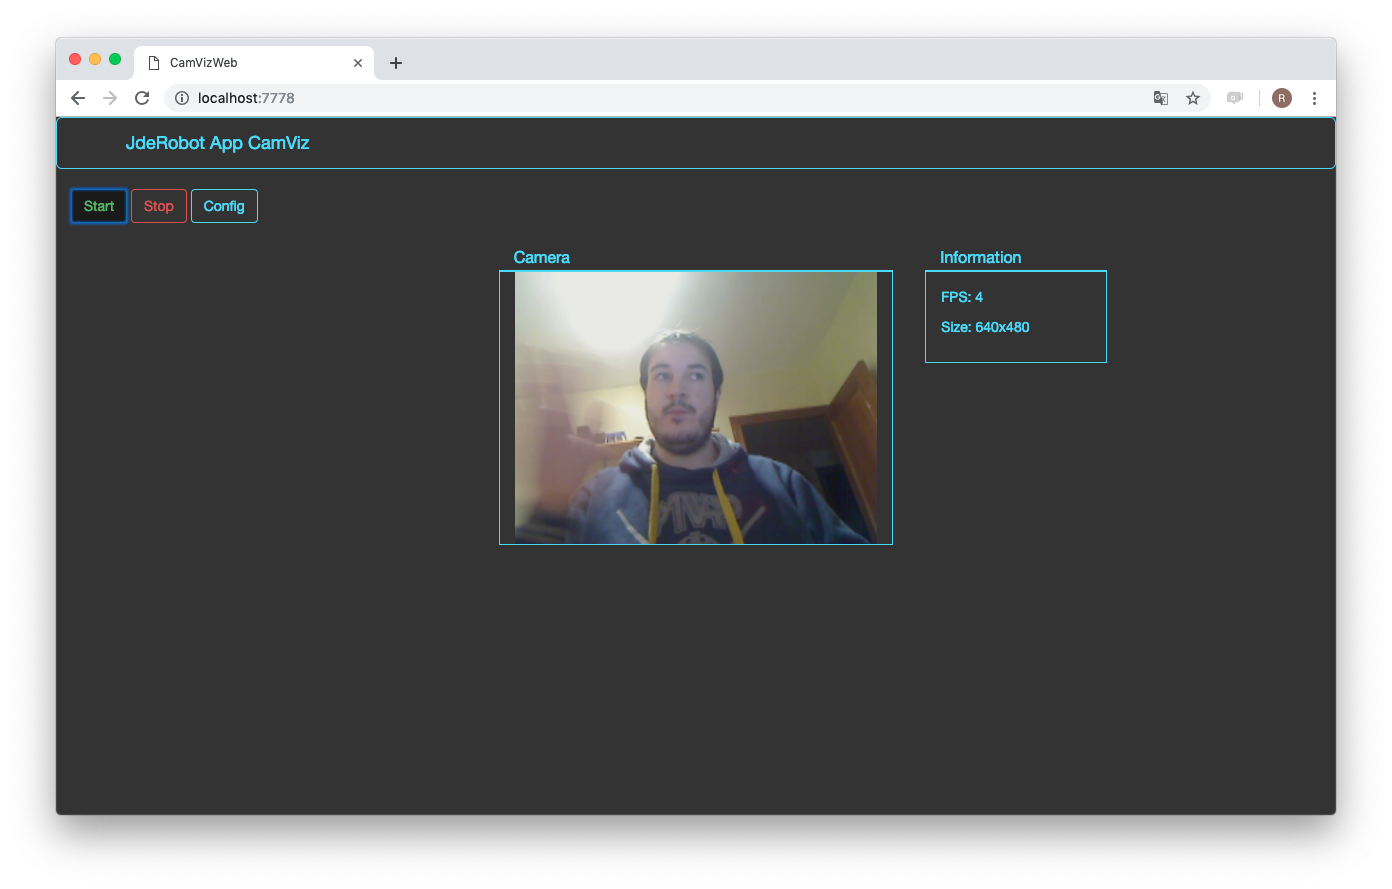
\includegraphics[width=0.8\textwidth]{figures/camviznode.png}
    		\caption{CamVizWeb ejecutado en un navegador web}
		\label{fig.camviznode}
		\end{center}
\end{figure}
\begin{figure}[H]
  \begin{center}
    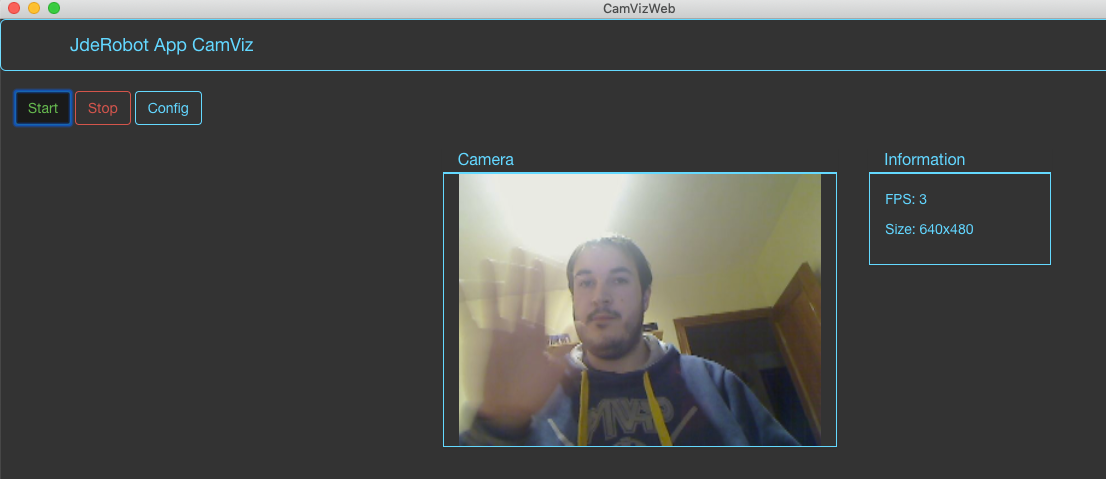
\includegraphics[width=0.8\textwidth]{figures/camvizelectron.png}
    		\caption{CamVizWeb ejecutado en Electron}
		\label{fig.camvizelectron}
		\end{center}
\end{figure}

\section{TurtlebotVizWeb}
Se trata de un visor y teleoperador para robots del tipo Turtlebot, desarrollado con tecnologías web, que usa los middleware de comunicación ICE y ROS y pude ser ejecutados con Electron o en un navegador web.

\subsection{Diseño}
La versión previa de esta herramienta solo contaba con ICE como \textit{middleware} de comunicación, por lo que al igual que ocurría con el caso de CamVizWeb, esto límitaba el uso de esta herramienta a Turtlebots que fueran capaces de comunicarse con ICE. Sin embargo, ahora será capaz también de conectarse con aquellos que se comuniquen mediante ROS. La figura 4.9 muestra el diagrama de bloques previo del sistema y la figura 4.10 muestra el diagrama tras la mejora realizada en este trabajo.

\begin{figure}[H]
  \begin{center}
    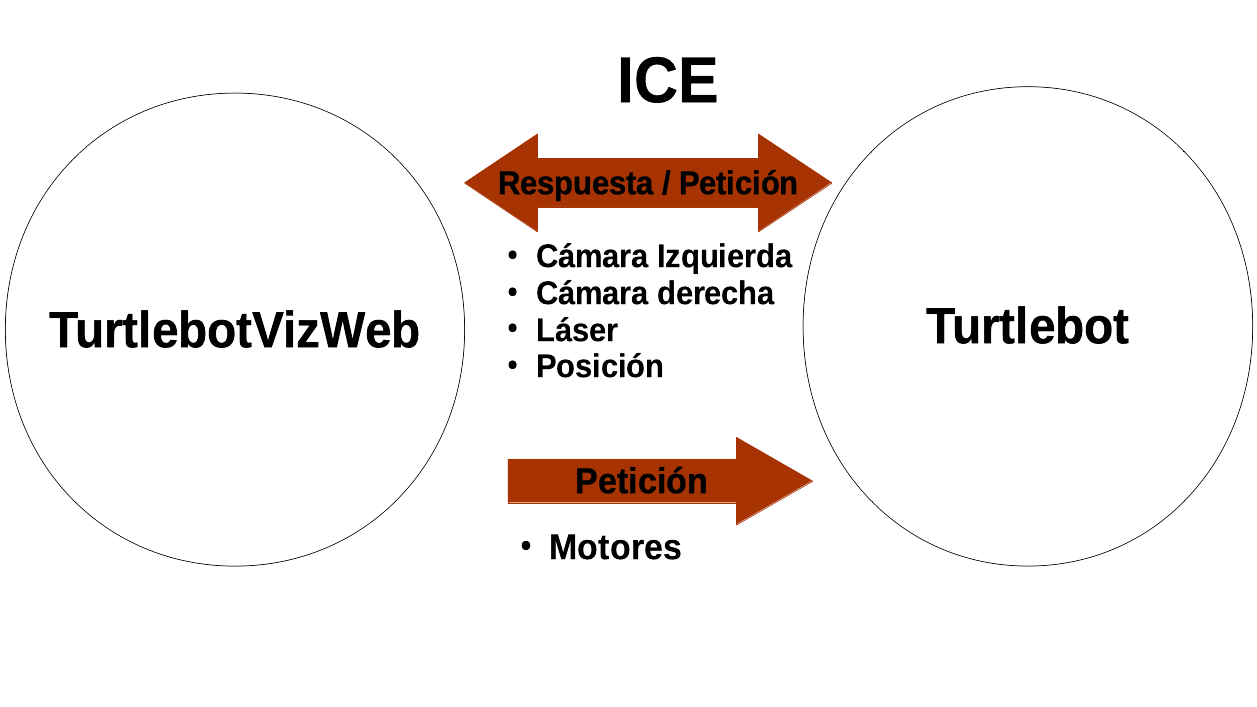
\includegraphics[width=0.8\textwidth]{figures/Turtlebot1.png}
		\caption{Diagrama de bloques previo del sistema}
		\label{fig.esquematurtlebot1}
		\end{center}
\end{figure}

\begin{figure}[H]
  \begin{center}
    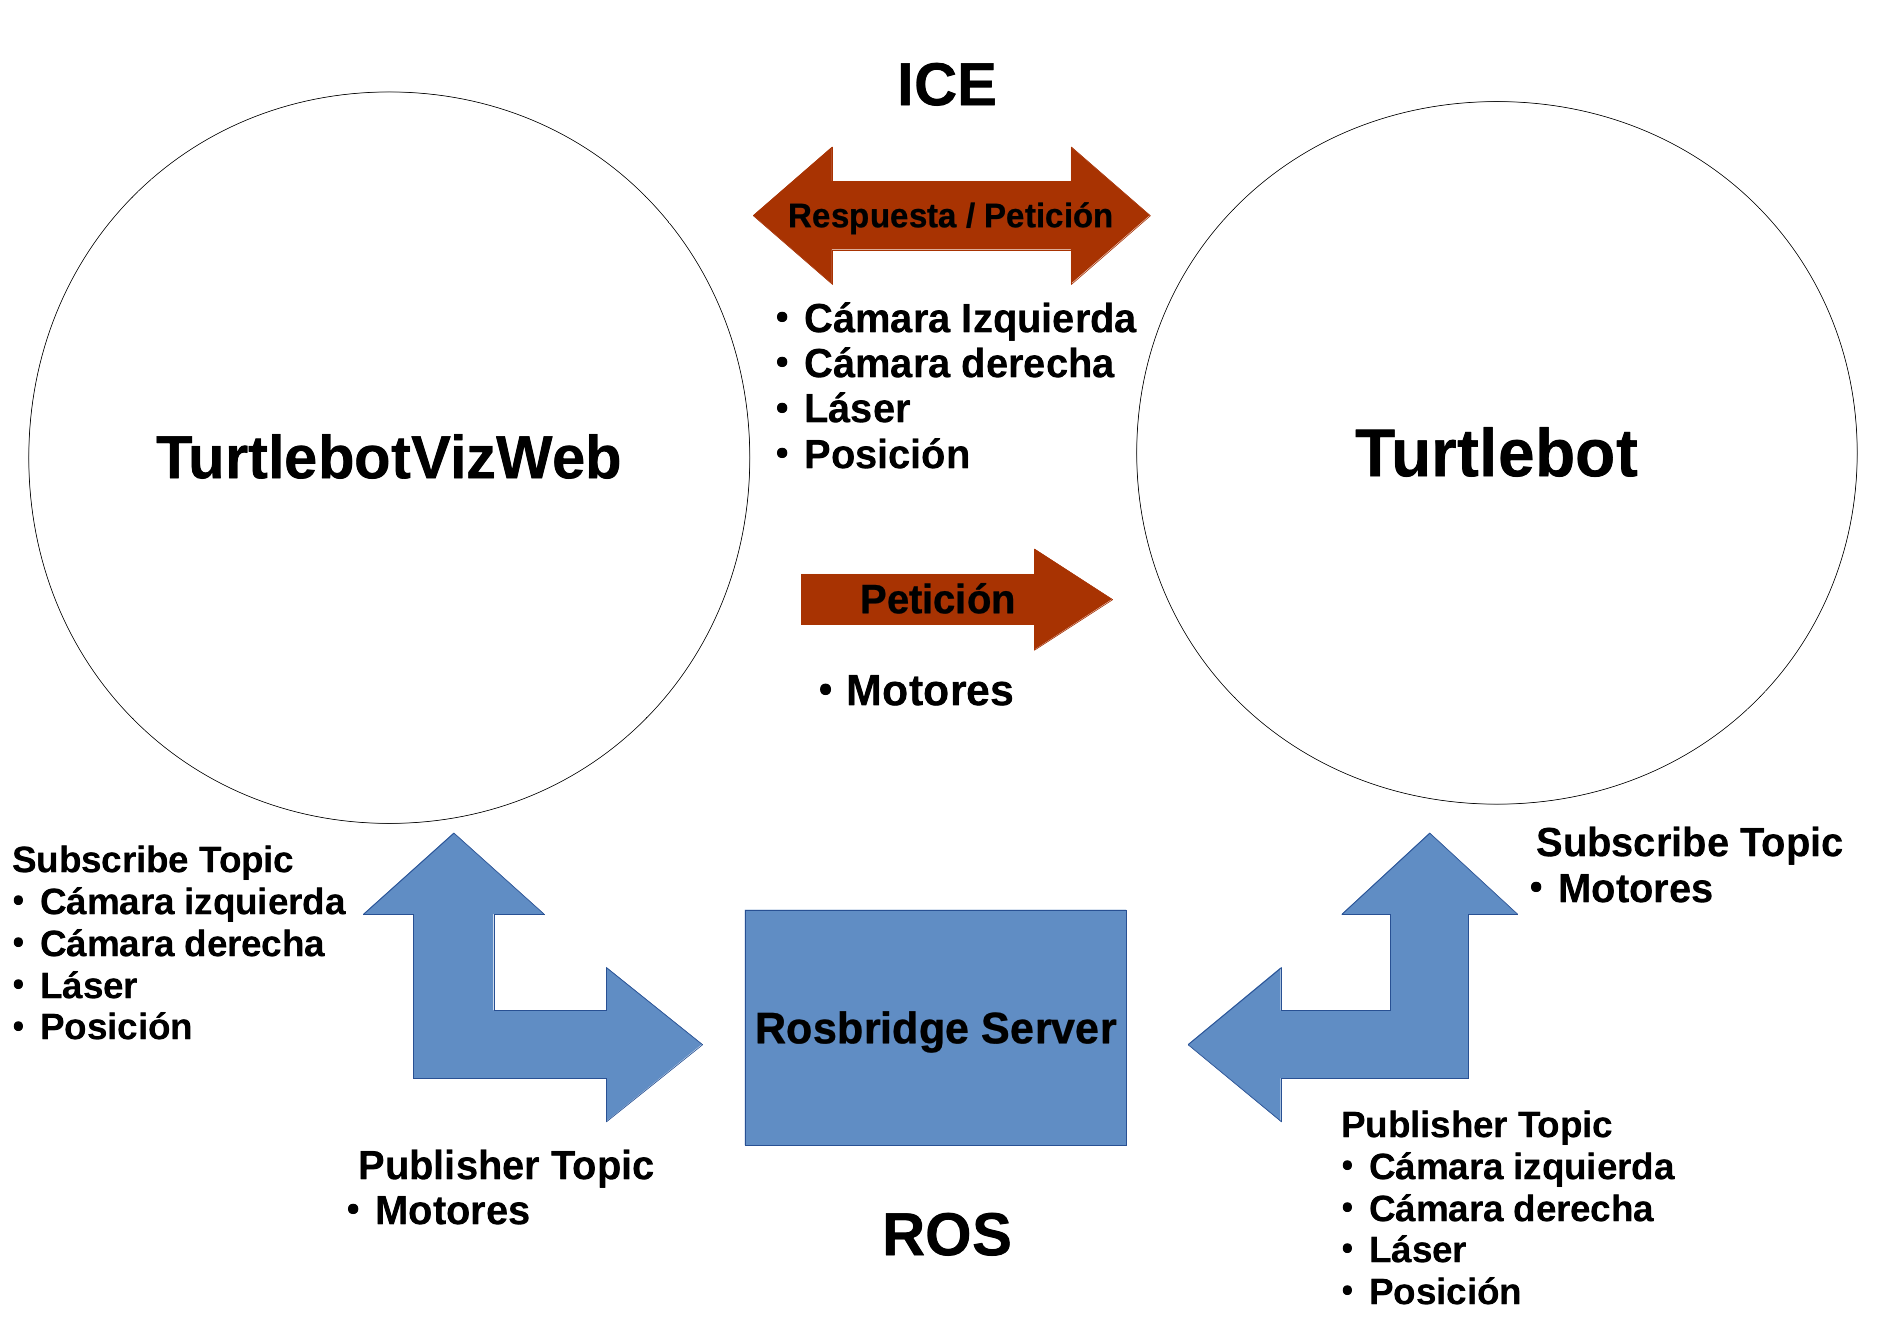
\includegraphics[width=0.8\textwidth]{figures/Turtlebot2.png}
		\caption{Diagrama de bloques actual del sistema}
		\label{fig.esquematurtlebot2}
		\end{center}
\end{figure}

En la figura 4.11 muestra la estructura de la aplicación previa de una manera más detallada, mientras que la figura 4.12 muestra la estructura tras realizar la modificación.

\begin{figure}[H]
  \begin{center}
    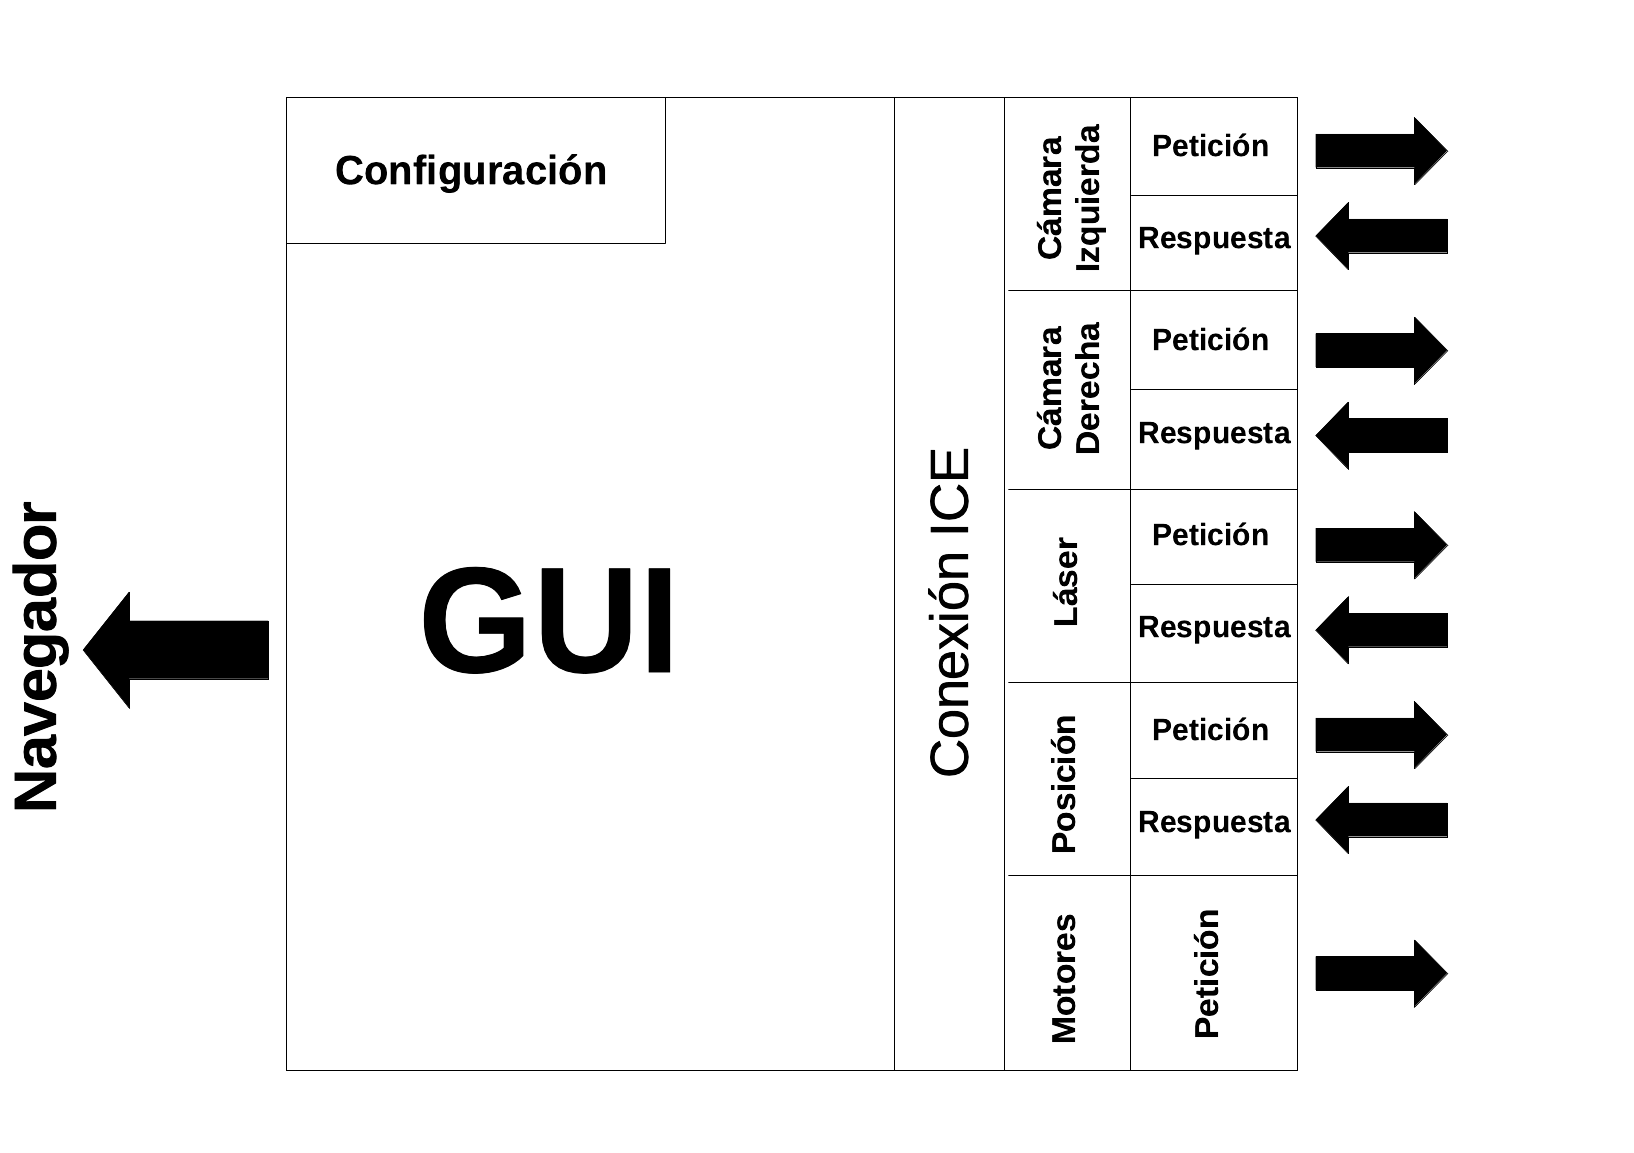
\includegraphics[width=0.8\textwidth]{figures/estrucuturaturtlebotviz1.png}
		\caption{Estructura previa de la herramienta}
		\label{fig.estructuracamviz2}
		\end{center}
\end{figure}

\begin{figure}[H]
  \begin{center}
    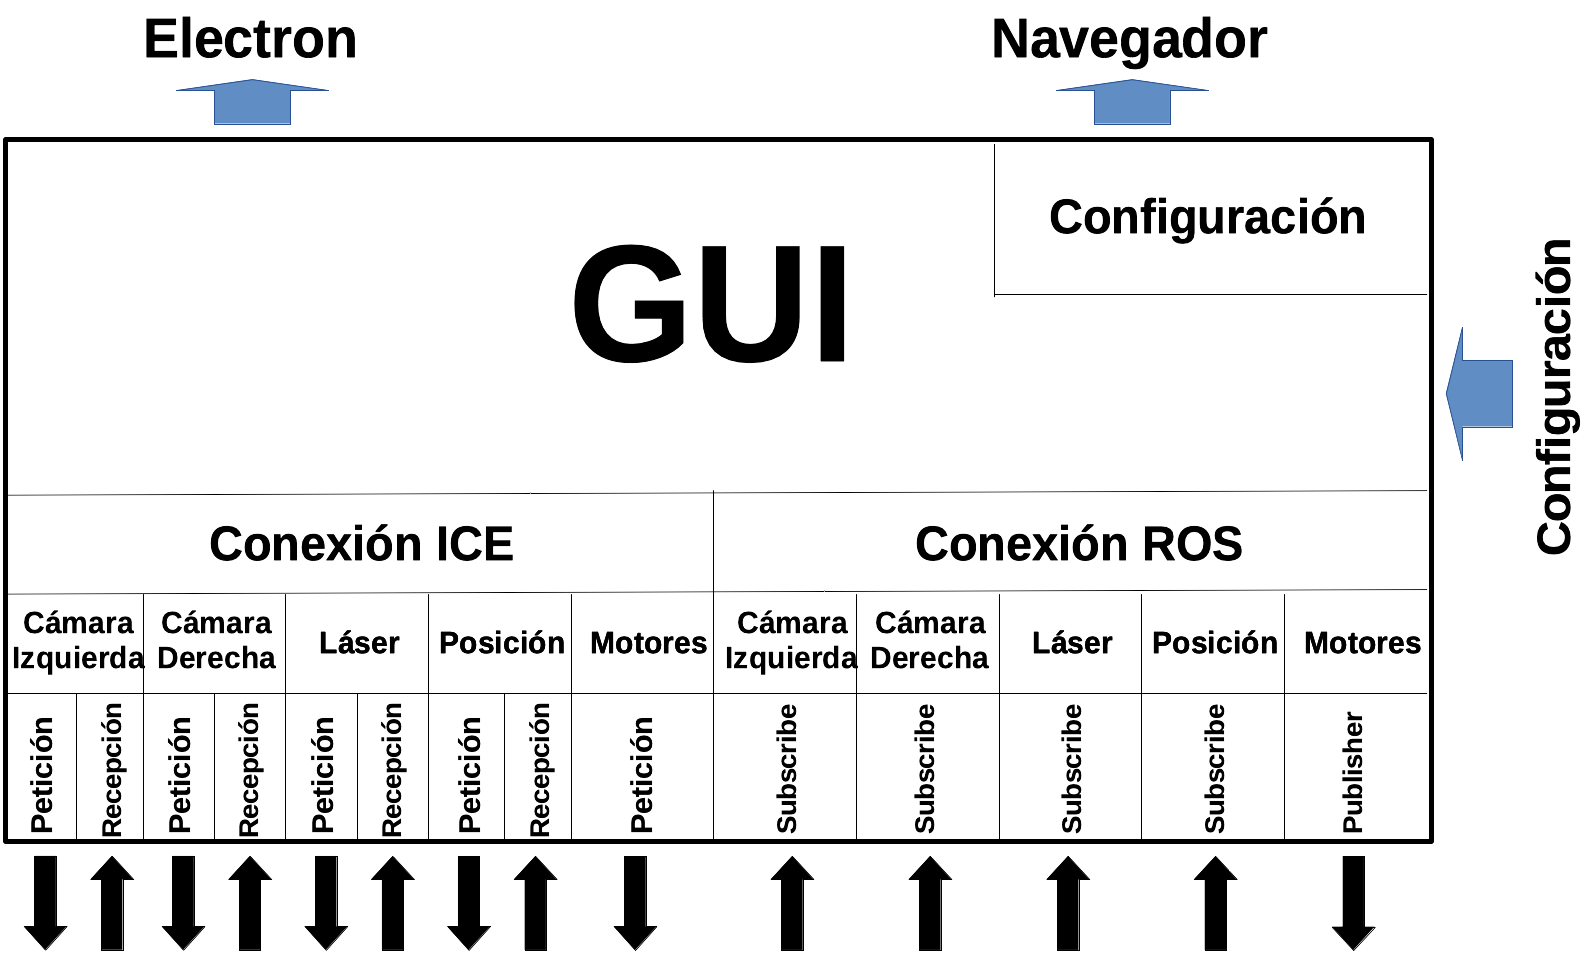
\includegraphics[width=0.8\textwidth]{figures/estrucuturaturtlebotviz2.png}
		\caption{Estructura actual de la herramienta}
		\label{fig.estructuracamviz2}
		\end{center}
\end{figure}

La herramienta esta dividida en dos partes: la interfaz gráfica y las conexiones. La interfaz gráfica contiene los elementos necesarios para visualizar los datos recibidos y teleoperar el turtlebot, además de contener un menu para realizar la configuración en tiempo de ejecución del visor.

La conexión se realiza mediante ICE o ROS. La conexión mediante ICE es la existente previamente en la aplicación, por lo que no se profundiza en la explicación de su funcionamiento, únicamente se indica que se solicitan cuatro mensajes al turtlebot: imagen de la cámara izquierda, imagen de la cámara derecha, datos del sensor láser y posición actual. Por otro lado, desde la propia herramienta se envía un mensaje con la información de los motores para teleoperar el robot (velocidad lineal y velocidad angular).

En el caso de ROS, se utiliza los \textit{subscribe} para recibir los mensajes procedentes del robot y los \textit{publisher} para transmitir la información de los motores. Teniendo en cuenta la información que se necesita, se realizan cuatro \textit{subscribe} (al igual que las peticiones ICE que se realizan) y un \textit{publisher}.

Por otro lado, al igual que para el visor CamVizWeb, se le añade la posibilidad de ejecutarse mediante el entorno Electron y la configuración previa mediante un archivo externo en formato ``YAML''.

\subsection{Interfaz gráfica}
La interfaz gráfica se vuelve a mantener la existente previamente realizando las modificaciones necesarias para realizar la conexión mediante el middleware ROS. La interfaz la forma cinco elementos \texttt{Canvas} de HTML5 y cuatro botones.
\begin{itemize}
\item \texttt{Canvas} para mostrar las imágenes de la cámara izquierda
\item \texttt{Canvas} para mostrar las imágenes de la cámara derecha
\item \texttt{Canvas} para mostrar los datos del sensor láser
\item \texttt{Canvas} para mostrar el posicionamiento del robot en 3D. Esta vista puede activarse y desactivarse manualmente mediante un botón.
\item \texttt{Canvas} con el teleoperador del robot.
\item Botón de arranque de la conexión.
\item Botón para parar la conexión.
\item Botón para abrir el menú de configuración.
\item Botón para parar el movimiento del robot.
\end{itemize}

Esta interfaz se puede visualizar en la figura 4.13.

\begin{figure}[H]
  \begin{center}
    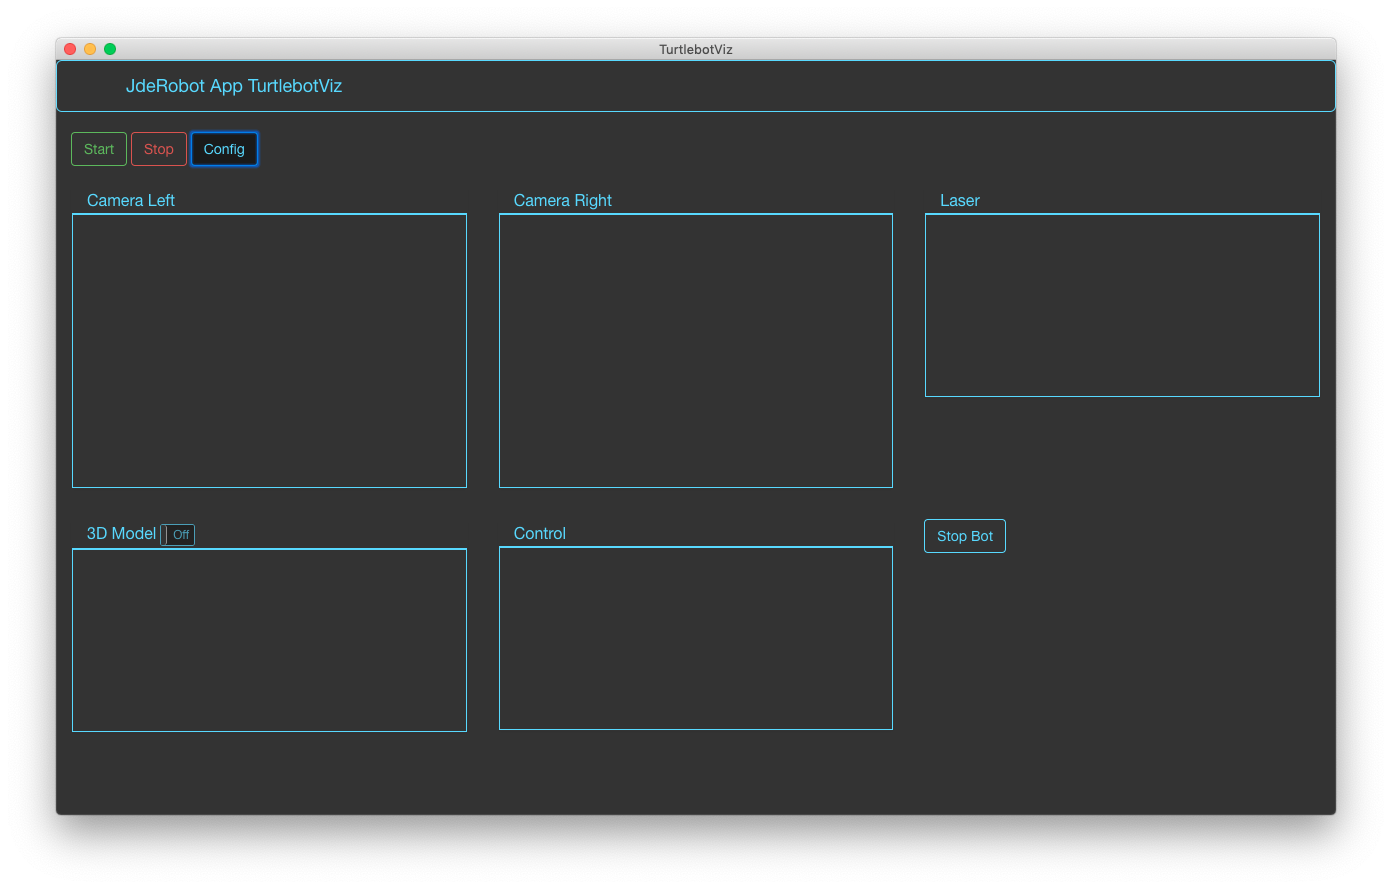
\includegraphics[width=0.8\textwidth]{figures/interfazturtlebotviz.png}
		\caption{Interfaz gráfica de TurtlebotVizWeb}
		\label{fig.iterfazturtlebotviz}
		\end{center}
\end{figure}

Para poder configurar la conexión mediante ROS, se vuelve a añadir un formulario con dos botones al menú de configuración para permitir en tiempo de ejecución elegir. Esto se realiza mediante el código HTML del cuadro 4.10.

\begin{lstlisting}[caption= Formulario para seleccionar el \textit{middleware} de comunicación, label=cod.formularioturtlebot]
<form class="form-inline">
      <button id="DfIce" type="button">Ice</button>
      <button id="DfRos" type="button">Ros</button>
</form>
\end{lstlisting}

En la figura 4.14 se muestra el nuevo menú de configuración.

\begin{figure}[H]
  \begin{center}
    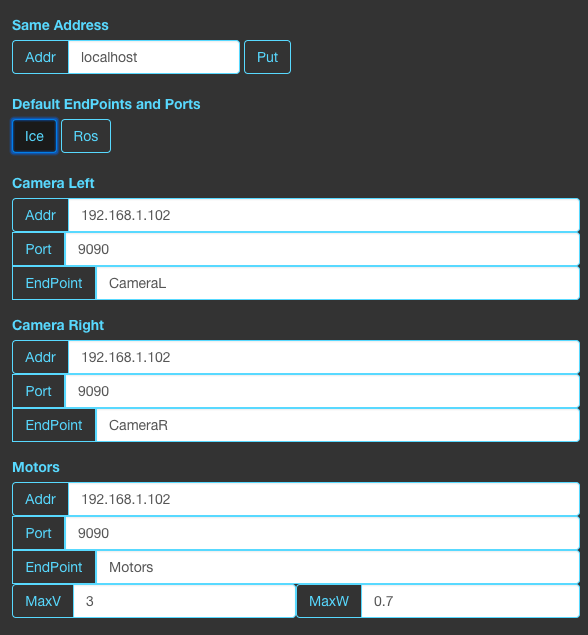
\includegraphics[width=0.8\textwidth]{figures/configturtlebot.png}
		\caption{Menu de configuración de TurtlebotVizWeb}
		\label{fig.configturtlebot}
		\end{center}
\end{figure}

\subsection{Conexiones}
La herramienta se ha modificado para que además de conexiones ICE, sea capaz de aceptar conexiones ROS, de manera que el funcionamiento sea igual de eficiente en ambos casos.

En su versión ICE, se desarrolló un \textit{API} (interfaz de programación de aplicaciones) con los métodos y objetos necesarios para realizar las conexiones ICE, la petición de cada mensaje (o el envío del mensaje para el caso de los motores) y el manejador de las respuestas desde el turtlebot. Por tanto, para el caso de la comunicación con ROS, se va a utilizar también el mismo \textit{API} incorporando los métodos y objetos necesarios para su funcionamiento y que se explican a continuación.

\subsubsection{Establecimiento de la conexión}
Lo primero que hay que indicar es que se realiza una conexión por cada tipo de mensaje que se desea recibir o transmitir. Cada conexión es un objeto de la \textit{API} con su constructor y métodos correspondientes, a excepción de la información de las cámaras que se utiliza el mismo objeto tanto para la cámara izquierda como para la derecha. Por tanto, se tendrán cuatro objetos diferentes dentro de la API que son \texttt{API.CameraRos, API.LaserRos, API.MotorsRos y API.Pose3DRos}, correspondiendo a las cámaras, al sensor láser, a los motores y a la posición del robot respectivamente.

Estos objetos se crean pasándoles por parámetro la información acerca de la conexión (dirección IP, puerto y \textit{topic} al que se debe subscribir), para que cuando se llame al método \texttt{connect} de cada objeto, se pueda realizar la conexión satisfactoriamente.

En el cuadro 4.11 se muestra como se define uno de estos objetos y el método para establecer la conexión. El resto de objetos se realiza de la misma manera.

\begin{lstlisting}[caption= Establecimiento de la conexión ROS , label=cod.conexionturtlebot]
API.CameraRos = function (config) {
	 var conf = config || {};
	 this.ros;
	 var self = this;
   	 this.connect = function (topic){
	
        self.ros = new ROSLIB.Ros({
            url : "ws://"+config.server.dir+":"+config.server.port
         });

         self.ros.on('connection', function() {
             console.log("Connect websocket Camera");
         });
         
        self.ros.on('error', function(error) {
            console.log("Error to connect websocket");
        });
}
...
}
\end{lstlisting}

Como se puede ver, la conexión se realiza de la misma forma que se explica en la sección 4.1.3.1, acerca de la conexión ROS del visor CamVizWeb. La única diferencia es que en esta ocasión en lugar de usar una variable global para toda conexión ROS mediante \texttt{self.ros}, ya que como se ha indicado anteriormente, cada objeto tendrá su propia conexión. Por otro lado, el método \texttt{connect} se define como \texttt{this.connect = function(config)} por la misma razón, es decir cada objeto tiene su propio método \texttt{connect} que se invocará cuando se inicialice cada conexión. Esta inicialización se realiza mediante el código del cuadro 4.12.

\begin{lstlisting}[caption= Creación de cada uno de los objetos de la \textit{API} y su posterior inicialización, label=cod.objetoapiturtlebot]
...
laser= new API.LaserRos(configlaser);
motors= new API.MotorsRos(configmotors);
cameraleft = new API.CameraRos (configcaml);
cameraright = new API.CameraRos(configcamr);
pose3d = new API.Pose3DRos(configpos);
    
laser.connect();
motors.connect();
cameraleft.connect();
cameraright.connect();
pose3d.connect();
...
\end{lstlisting}
Las cinco primeras línea de código corresponden a la creación de los objetos, como se puede ver su número coincide con los mensajes que se van a recibir y enviar. Las siguientes cinco líneas corresponden a la invocación del método para inicializar la conexión. En cada caso se invoca a su propio método \texttt{connect}, lo que es posible gracias a que se crea como se ha indicado anteriormente.

\subsubsection{Estructura de los mensajes}
Como se ha indicado en la sección 4.2.1, se van a utilizar cuatro mensajes de los tipos predeterminados de ROS y definidos en su documentación\footnote{\url{http://wiki.ros.org/common_msgs}}. Para definirlos se va a utilizar lo mismo que se explicó en la sección 4.1.3.2.

Para obtener las imágenes de las cámaras, al igual que en el visor CamVizWeb, se va a usar el tipo \texttt{sensor\_msgs/CompressedImage} y se define como se muestra en el cuadro 4.13 y se incluye dentro del método \texttt{connect} de \texttt{API.CameraRos}.

\begin{lstlisting}[caption= Definición del mensaje para la información de las cámaras, label=cod.mensajecamturtle]
self.roscam = new ROSLIB.Topic({
            ros : self.ros,
            name : config.topic,
            messageType : "sensor_msgs/CompressedImage"
});
\end{lstlisting}

El mensaje para obtener el sensor láser es del tipo \texttt{sensor\_msgs/LaserScan}, que nos ofrece toda la información necesaria para poder representar lo obtenido mediante el driver incorporado en el turtlebot. En el cuadro 4.14 se muestra la definición de este mensaje y forma parte del método \texttt{connect} de \texttt{API.LaserRos}.

\begin{lstlisting}[caption= Definición del mensaje para obtener la información del sensor láser, label=cod.mensajelaserturtle]
self.roslaser = new ROSLIB.Topic({
            ros : self.ros,
            name : config.topic,
            messageType : "sensor_msgs/LaserScan"
});
\end{lstlisting}

Para definir el mensaje que proporciona la posición del robot en cada momento se va a utilizar \texttt{nav\_msgs/Odometry}, que proporciona la posición mediante la clase ``Pose3D''. Esta clase esta formada por las coordenadas ``X'', ``Y'' y ``Z'' para ubicar el robot, la coordenada homogénea ``h'' y los cuaterniones ``q0'', ``q1'', ``q2'' y ``q3''  para obtener su orientación. En el cuadro 4.15 se muestra la definición de este mensaje, que como en los casos anteriores se define dentro del método \texttt{connect} del objeto \texttt{API.Pose3DRos}.

\begin{lstlisting}[caption= Definición del mensaje para obtener el posicionamiento del turtlebot, label=cod.mensajeposeturtle]
self.rospose = new ROSLIB.Topic({
		ros : self.ros,
		name : config.topic,
		messageType : "nav_msgs/Odometry"
});
\end{lstlisting}

Ahora solo falta por definir el único mensaje que se transmite desde el visor mediante \textit{Publisher}. Este mensaje es el que enviara el movimiento indicado con el teleoperador al turtlebot y es del formato de ROS \texttt{geometry\_msgs/Twist}. Este tipo de ROS permite transmitir tanto la velocidad lineal en tres dimensiones como la velocidad angular en las mismas tres dimensiones. En el cuadro 4.16 se muestra como se define este mensaje dentro del método \texttt{connect} del objeto \texttt{API.MotorsRos}.

\begin{lstlisting}[caption= Definición del mensaje para transmitir el movimiento proporcionado por el teleoperador, label=cod.mensajemotorturtle]
self.rosMotors = new ROSLIB.Topic({
		ros : self.ros,
		name : config.topic,
		messageType : "geometry_msgs/Twist"
});
\end{lstlisting}

\subsubsection{Subscripción a los \textit{Topic} y tratamiento de la información}
Cada tipo de mensaje recibido es tratado de manera independiente. Se ha definido el método \texttt{startStreaming} para cada uno de los objetos de la API mencionados en la sección 4.2.3.1.

\paragraph{Subscripción y tratamientos de las cámaras}

Para el caso de las imágenes obtenidas de las cámaras, el tratamiento y subscripción es muy similar al explicado en la sección 4.1.3.3, por lo que no se vuelve a profundizar en ello, únicamente hacer hincapié en que un robot turtlebot cuenta con dos cámaras (izquierda y derecha), por lo que se tiene un \textit{Subscribe} para cada cámara y, por consiguiente, se tratan las imágenes recibidas de manera independiente. La figura 4.15 muestra la visualización de ambas cámaras.

\begin{figure}[H]
  \begin{center}
    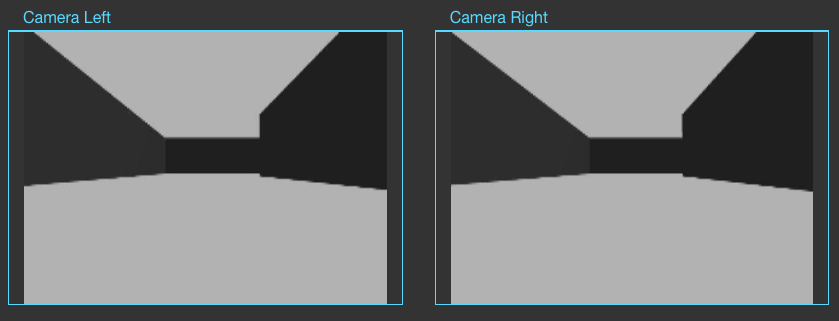
\includegraphics[width=0.8\textwidth]{figures/camarasturtle.png}
		\caption{Visualización de la información de las cámaras}
		\label{fig.camarasturtle}
		\end{center}
\end{figure}

\paragraph{Subscripción y tratamiento del sensor láser}

La subscripción del mensaje con el sensor láser se realiza de la misma forma que la cámara, sin embargo en este caso el tratamiento se realiza de manera diferente. Lo primero que hay que tener en cuenta es que el mensaje transmite la información acerca del ángulo mínimo y máximo del escaneo, el valor del rango mínimo y máximo, y el rango de datos. Con esta información se debe recrear el escaneo tanto en 2D como en 3D. Cabe indicar que el escaneo 3D solo se muestra en caso de que así se deseé, ya que únicamente se mostrará en el momento que se active la representación 3D del turtlebot en el visor.

\begin{lstlisting}[caption= Subscripción y tratamiento del mensaje para su visualización en 2D, label=cod.subslaser2D]
this.startStreaming = function(convertUpAxis,canv2dWidth, scale3d, model){
	self.roslaser.subscribe(function(message){
		var i,j;
		var numlaser = message.ranges.length;
		var dist =  message.ranges;
		var minAngle = message.angle_min;
		var maxAngle = message.angle_max;
		var minRange = message.range_min;
		var maxRange = message.range_max;
		var step = (maxAngle - minAngle) / numlaser;
		var array2d = [];
		var max = canv2dWidth/2;
		var center = {x:canv2dWidth/2 , y:canv2dWidth/2};
		for (i = 0; i< numlaser; i++ ){
			var ang = minAngle + i * step;
			var dd = calcNorm2DPoint (dist[i], maxRange, 
									ang, max, center,canv2dWidth);
			array2d[2*i] = dd.x;
			array2d[2*i+1] = dd.y;
		 }
		var laser = {}
		laser.distanceData = dist;
		laser.numLaser = numlaser;
		laser.maxAngle = maxAngle;
		laser.minAngle = minAngle;
		laser.maxRange = maxRange;
		laser.minRange = minRange;
		laser.canv2dData = array2d;
		drawLaser(laser,model,canv2dWidth);
	});
};
\end{lstlisting}

En el cuadro 4.17 se muestra como se realiza la subscripción y como se trata el mensaje recibido para visualizar el escaneo en 2D. Lo primero es obtener los datos del mensaje que se van a utilizar y se han indicado anteriormente. A partir e hay se define el tamaño y el centro de la recreación, así como el tamaño del barrido del sensor láser que es la resta del máximo y mínimo ángulo de escaneo dividido entre el total de ángulos escaneados. Obtenido este dato, se crea un bucle para representarlo de manera que cada iteración corresponde a cada ángulo escaneado. Dentro de cada iteración se obtiene el ángulo, se obtiene la coordenada x e y mediante la función \texttt{calcNorm2DPoint} que se muestra en el cuadro 4.18 y se almacena dentro del array que se visualizará. Finalmente todos los datos se almacenan en la variable \texttt{laser} y se invoca al método \texttt{drawLaser} que se explicará más adelante.

\begin{lstlisting}[caption= Calcular las coordenadas 2D, label=cod.lasercoor2d]
function calcNorm2DPoint (dist, maxRange, ang, max2d, center, width){
	var x;
	var y;
	var d = maxRange/max2d;
	if (dist == null){
		x = center.x - ((maxRange /d) * (Math.sin(ang)));
		y = center.y - ((maxRange /d) * (Math.cos(ang)));
	} else {
		x = center.x - ((dist /d) * (Math.sin(ang)));
		y = center.y - ((dist /d) * (Math.cos(ang)));
	 }
	 var a = {x:x,y:y};
	 return a;
}
\end{lstlisting}

En la figura 4.16 se muestra la visualización del láser en 2D.

\begin{figure}[H]
  \begin{center}
    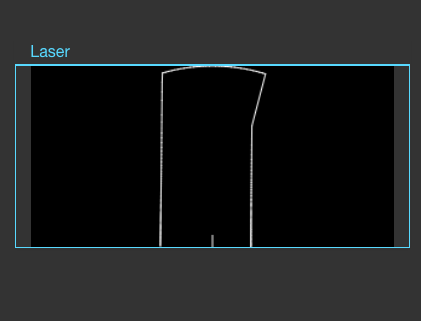
\includegraphics[width=0.8\textwidth]{figures/laser2dturtle.png}
		\caption{Visualización de la información del láser en 2D}
		\label{fig.laser2dturtle}
		\end{center}
\end{figure}

Para visualizar la información sobre el sensor láser en 3D, se amplia el método \texttt{startStreaming}.

\begin{lstlisting}[caption= Subscripción y tratamiento del mensaje para su visualización 3D label=cod.subslaser3D]
this.startStreaming = function(convertUpAxis,canv2dWidth, scale3d, model){
	self.roslaser.subscribe(function(message){
		...
		var array3d = [];
		j=9;
		var d1 = calc3dPoint (dist[0], maxRange, Math.PI, 
							convertUpAxis, scale3d);
		var d2 = calc3dPoint (dist[1], maxRange, Math.PI-Math.PI/numlaser, 
							convertUpAxis, scale3d);
		array3d[0] = d1.x;
		array3d[1] = d1.y;
		array3d[2] = d1.z;
		array3d[3] = 0;
		array3d[4] = 0;
		array3d[5] = 0;
		array3d[6] = d2.x;
		array3d[7] = d2.y;
		array3d[8] = d2.z;
		for (i=2;i< numlaser; i++){
			ang = (i*Math.PI/numlaser);
			var d = calc3dPoint (dist[i], maxRange, ang, 
								convertUpAxis, scale3d);
			array3d[j+0] = array3d[j-3];
			array3d[j+1] = array3d[j-2];
			array3d[j+2] = array3d[j-1];
			array3d[j+3] = 0;
			array3d[j+4] = 0;
			array3d[j+5] = 0;
			array3d[j+6] = d.x;
			array3d[j+7] = d.y;
			array3d[j+8] = d.z;
			j = j + 9;
		}
		laser.array3dData = array3d;
		drawLaser(laser,model,canv2dWidth);	
	});
};
\end{lstlisting}

En el cuadro 4.19 se muestra el código añadido al método para poder representar el escaneo en 3D. Lo primero que hay que tener en cuenta es la forma en que se representa en 3D el escaneo. Para representar el turtelbot y el escaneo en 3D se utiliza \texttt{WebGL} y la biblioteca \texttt{Three.js}. Como se explicará en el método \texttt{drawLaser} se utiliza el objeto \texttt{new THREE.BufferGeometry()} para representar el escaneo. A este objeto hay que indicarle las componentes de cada vector, divide el \textit{array} de datos pasados en vectores y dibuja triángulos utilizando tres vectores consecutivos del \textit{buffer}. En este caso, el vector va a contar con 3 componentes ya que es en 3D (``x'', ``y'' y ``z''), y cada triangulo está dibujado mediante tres vertices que son dos puntos escaneados por el láser y el origen de coordenadas.

Indicado esto, ya se tiene los conocimientos previos para entender el código del cuadro 4.19. Lo primero que se hace es calcular los dos primeros puntos del escaneo mediante la función del cuadro 4.20 y se almacenan en el \textit{array}. Como se puede ver, se divide en grupos de nueve datos, de manera que en los tres primeros datos se almacenan las coordenadas del primer punto del escaneo, en los siguientes tres se almacena el origen de coordenadas y en los tres últimos el segundo punto del escaneo. Calculada la representación de los dos primeros puntos obtenidos mediante el sensor láser, se define un bucle para la representación del resto de puntos, siendo cada iteración cada uno de los ángulos escaneados. Creado el \textit{array} se añade a la variable \texttt{laser} utilizada para el láser en 2D y que se pasa por parámetros al método \texttt{drawLaser}.


\begin{lstlisting}[caption= Calcular las coordenadas 3D, label=cod.lasercoor3d]
function calc3dPoint (dist,maxdist, ang, convertUpAxis, scale){
	var a;
	var x;
	if (dist == null){
		a = scale * maxdist * Math.cos(ang);
		x = scale * maxdist * Math.sin(ang);
	 } else {
	 	a = scale * dist * Math.cos(ang);
		x = scale * dist * Math.sin(ang);
	 }
	 if (convertUpAxis){
	 	return {x:x,y:0,z:a};
	} else {
		return {x:x,y:a,z:0};
	}
}
\end{lstlisting}

Tras obtener todos los datos necesarios para representar la información obtenida por el sensor láser, se invoca al método \texttt{drawLaser}.

\begin{lstlisting}[caption= Método para bibujar el escaneo del sensor láser, label=cod.dibujarlaser]
function drawLaser(laser, model){
	var dist = laser.canv2dData;
	var lasercanv = document.getElementById("laser");
	var ctx = lasercanv.getContext("2d");
	ctx.beginPath();
	ctx.clearRect(0,0,lasercanv.width,lasercanv.height);
	ctx.fillRect(0,0,lasercanv.width,lasercanv.height);
	ctx.strokeStyle="white";
	ctx.moveTo(dist[0], dist[1]);
	for (var i = 2;i<dist.length; i = i+2 ){
		ctx.lineTo(dist[i], dist[i+1]);
	}
	ctx.moveTo(lasercanv.width/2, lasercanv.height);
	ctx.lineTo(lasercanv.width/2, lasercanv.height-10);
	ctx.stroke();
	
	if (model.active){
		var geometry = new THREE.BufferGeometry();
		geometry.addAttribute( 'position', 
			new THREE.BufferAttribute(new Float32Array(laser.array3dData),3));
		var material = new THREE.MeshBasicMaterial( { color: 0x00ff00 } );
		material.transparent = true;
		material.opacity=0.5;
		material.side = THREE.DoubleSide;
		var las = new THREE.Mesh( geometry, material );
		if (model.laser){
			model.robot.remove(model.laser);
		};
		model.robot.add(las);
		model.laser = las;
	}
}
\end{lstlisting}

En el cuadro 4.21 se muestra el método para dibujar el escaneo del láser. El escaneo en 2D se dibuja sobre el elemento de HTML5 \texttt{Canvas} utilizando sus métodos para representar gráficos. El escaneo en 3D se realiza, como se ha indicado anteriormente, mediante la biblioteca de \texttt{WebGL} \texttt{Three.js} y el objeto \texttt{THREE.BufferGeometry()}, pero únicamente se mostrará en caso de que este activa la visualización del modelo 3D. La figura 4.17 muestra el escaneo realizado por el sensor láser en 3D.

\begin{figure}[H]
  \begin{center}
    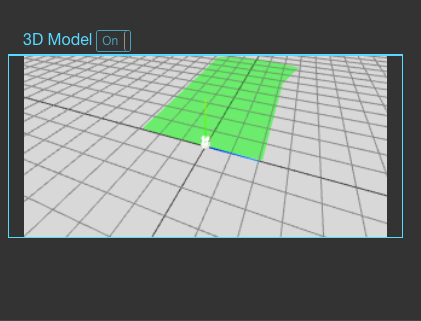
\includegraphics[width=0.8\textwidth]{figures/laser3dturtle.png}
		\caption{Visualización de la información del láser en 3D}
		\label{fig.laser3dturtle}
		\end{center}
\end{figure}

\paragraph{Subscripción y tratamiento de la odometría}

El último \textit{topic} al que se subscribe es el encargado de proporcionar el mensaje con la posición y orientación del turtlebot mediante la clase ``Pose3D''. Esta clase, que se detallará más extensamente en la sección 5.5.2.3, proporciona la posición a través de las coordenadas ``x'', ``y'' y ``z'', y la orientación mediante los cuaterniones ``q0'', ``q1'', ``q2'' y ``q3'' tras realizar las conversiones oportunas mediante una serie de fórmulas matemáticas.

Al igual que se realiza para el sensor láser en 3D, únicamente se utiliza este mensaje en caso de que se deseé mostrar la representación en 3D del turtlebot mediante WebGL (aunque si se realiza la subscripción al \textit{topic} para que cuando se deseé mostrar no haya retardos). La subscripción se realiza de la misma forma que en los casos anteriores, es decir mediante el método \texttt{startStreaming}

\begin{lstlisting}[caption= Subscripción y tratamiento del mensaje para obtener la posición, label=cod.pose3d]
this.startStreaming = function(model){
	self.rospose.subscribe(function(message){
		if (lastPose != message.pose){
			if (model.active) {
				var orientation = getPose3D(message.pose.pose.orientation);
				model.robot.position.set(message.pose.pose.position.x, 
					message.pose.pose.position.z, -message.pose.pose.position.y);
				model.robot.rotation.y=(orientation.yaw);
				model.robot.updateMatrix();
			}
		}
		lastPose = message.pose;
	});
};
\end{lstlisting}

En el cuadro 4.22 se puede visualizar como se realiza la subscripción. La variable \texttt{lastpose} se define en el constructor de objeto \texttt{API.Pose3DRos} y toma el valor de la posición obtenida en el anterior mensaje recibido. Con esta variable se detecta cuando la posición ha sufrido cambios de modo que se desechen los mensajes que no envíen información sobre un cambio en la posición. En caso que el mensaje recibido transmita información sobre una nueva ubicación, se comprueba si esta activa la representación 3D del robot. Si así lo fuera, se realiza la conversión de los cuaterniones para obtener la orientación del robot que se explicará en la sección 5.5.2.3. Tras esto, se posición la representación del turtlebot en la nueva ubicación, teniendo en cuenta que el sistema de coordenadas utilizado por WebGL no es el mismo que el del robot, por lo que la coordenada ``y'' de WebGL corresponde a la coordenada ``z'' del robot, y la coordenada ``z'' de la representación corresponde a la ``-y'' del robot. Posteriormente se establece la nueva orientación, que en el caso del turtlebot solo rotara alrededor del eje vertical, por lo que solo es necesario indicar la orientación en el eje de coordenadas ``y''. Para finalizar, se actualiza la visualización de la representación del turtlebot y se almacena esta posición en la variable \texttt{lastPose} para indicar que es el último movimiento realizado tal y como se ha indicado anteriormente.

En la figura 4.17 donde se muestra el láser 3D, también se puede ver la representación del turtlebot que se visualiza en el visor.

\subsubsection{Publicación del mensaje con la información del teleoperador}

Tras describir como realizar la subscripción a los mensajes publicados por el turtlebot y posteriormente tratarlos para mostrar lo que se recibe, hay que explicar como se crear y posteriormente se publica el mensaje con la información de los motores.

Lo primero que hay que indicar que los motores se controlan mediante una interfaz creada usando WebGL y la biblioteca \texttt{Three.js}. Esta interfaz cuenta con una linea vertical y otra horizontal que se cruzan formando una cruz, y un circular para indicar el movimiento, de manera que la linea vertical marca el movimiento hacia delante y hacia detrás del robot (la velocidad lineal) y la linea horizontal hacia donde debe girar (la velocidad angular). En la figura 4.18 se muestra esta interfaz.

\begin{figure}[H]
  \begin{center}
    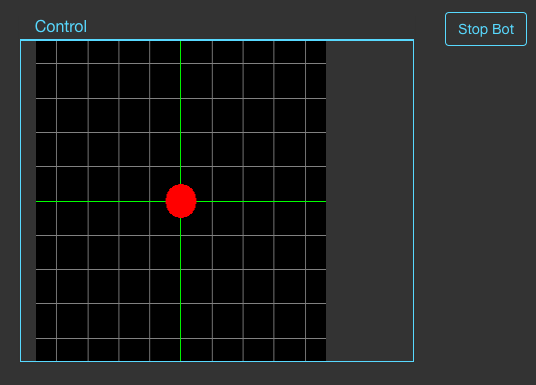
\includegraphics[width=0.8\textwidth]{figures/controlturtle.png}
		\caption{Interfaz para el control de los motores}
		\label{fig.controlturtle}
		\end{center}
\end{figure}

Indicado esto, para transmitir la información de los motores se ha creado el método \texttt{setMotors} dentro del objeto \texttt{API.MotorsRos}. A este método se le introducen como parámetros las información de la velocidad linea y la velocidad angular, y prepara el mensaje para que tenga la estructura del tipo predeterminado de ROS \texttt{geometry\_msgs/Twist}\footnote{\url{http://docs.ros.org/melodic/api/geometry_msgs/html/msg/Twist.html}} para posteriormente publicarlo mediante los \textit{Publisher} de ROS.

\begin{lstlisting}[caption= Preparación y publicación del mensaje con el control de los motores, label=cod.motores]
this.setMotors = function(v,w){
	var motorsMessage = new ROSLIB.Message({
		linear: v,
		angular: w
	});
	self.rosMotors.publish(motorsMessage);
	}
\end{lstlisting}

El código del cuadro 4.23 realiza la preparación y la publicación de los mensajes para transmitir la información de los motores al turtlebot. Primero se prepara el mensaje mediante la utilización del objeto de \textit{roslibjs} \texttt{ROSLIB.Message}, definiendo la velocidad lineal y angular con los parámetros introducidos en la invocación al método. Definido el mensaje a transmitir, se utiliza el método de \textit{roslibjs} \texttt{publish} introduciendo como parámetro el mensaje definido con la información de los motores.

Sin embargo, con este método solo se transmite un mensaje con el control de los motores, y lo que se desea es estar continuamente enviando esta información para que el turtlebot sepa en todo momento como se debe comportar. Para lograr esto, se utiliza el método de HTML \texttt{setInterval}\footnote{\url{https://www.w3schools.com/jsref/met_win_setinterval.asp}} que proporciona la ejecución de código cuando ha transcurrido el periodo de tiempo indicado.

\begin{lstlisting}[caption= Invocación cada milisegundo al método para publicar el mensaje con los motores, label=cod.setintervalTurtle]
setInterval(function (){
        motors.setMotors(v,w)
},1);
\end{lstlisting}

En el cuadro 4.24 se puede ver que cada milisegundo se invoca al método \texttt{setMotors} introduciendo la velocidad lineal y angular establecida en ese momento para que se publique y el turtlebot pueda recibirla.

\subsection{Configuración}
Al igual que en el visor CamVizWeb, la configuración puede ser realizada via un fichero externo del tipo ``YAML'' o en tiempo de ejecución con el menu configuración de la interfaz gráfica.

Los parámetros configurables para este visor son los siguientes:
\begin{itemize}
\item \textit{Middleware} utilizado para realizar la comunicación. Por defecto es ICE.
\item Dirección IP para conectar el visor a la cámara izquierda del turtlebot. Por defecto ``localhost''.
\item Puerto para conectar el visor a la cámara izquierda del turtlebot. Por defecto es ``9090''.
\item Endpoint para conectar el visor a la cámara izquierda del turtlebot. Este parámetro solo se utiliza para realizar la comunicación mediante ICE, por lo que si se indica ROS, se ignora. Por defecto es ``CameraL''.
\item Topic para conectar el visor a la cámara izquierda del turtlebot. Este parámetro solo se utiliza para realizar la comunicación mediante ROS, por lo que se indica ICE, se ignora. Por defecto es ``/TurtlebotROS/cameraL/image\_raw/compressed''.
\item Dirección IP para conectar el visor a la cámara derecha del turtlebot. Por defecto ``localhost''.
\item Puerto para conectar el visor a la cámara derecha del turtlebot. Por defecto es ``9090''.
\item Endpoint para conectar el visor a la cámara derecha del turtlebot. Este parámetro solo se utiliza para realizar la comunicación mediante ICE, por lo que si se indica ROS, se ignora. Por defecto es ``CameraR''.
\item Topic para conectar el visor a la cámara derecha del turtlebot. Este parámetro solo se utiliza para realizar la comunicación mediante ROS, por lo que se indica ICE, se ignora. Por defecto es ``/TurtlebotROS/cameraR/image\_raw/compressed''.
\item Dirección IP para conectar el visor con los motores del turtlebot. Por defecto ``localhost''.
\item Puerto para conectar el visor con los motores del turtlebot. Por defecto es ``9090''.
\item Endpoint para conectar el visor con los motores del turtlebot. Este parámetro solo se utiliza para realizar la comunicación mediante ICE, por lo que si se indica ROS, se ignora. Por defecto es ``Motors''.
\item Topic para conectar el visor con los motores del turtlebot. Este parámetro solo se utiliza para realizar la comunicación mediante ROS, por lo que se indica ICE, se ignora. Por defecto es ``/turtlebotROS/mobile\_base/commands/velocity''.
\item Dirección IP para conectar el visor a la odometría del turtlebot. Por defecto ``localhost''.
\item Puerto para conectar el visor a la odometría del turtlebot. Por defecto es ``9090''.
\item Endpoint para conectar el visor a la odometría del turtlebot. Este parámetro solo se utiliza para realizar la comunicación mediante ICE, por lo que si se indica ROS, se ignora. Por defecto es ``Pose3D''.
\item Topic para conectar el visor a la odometría del turtlebot. Este parámetro solo se utiliza para realizar la comunicación mediante ROS, por lo que se indica ICE, se ignora. Por defecto es ``/turtlebotROS/odom''.
\item Dirección IP para conectar el visor al sensor láser del turtlebot. Por defecto ``localhost''.
\item Puerto para conectar el visor al sensor láser del turtlebot. Por defecto es ``9090''.
\item Endpoint para conectar el visor al sensor láser del turtlebot. Este parámetro solo se utiliza para realizar la comunicación mediante ICE, por lo que si se indica ROS, se ignora. Por defecto es ``Laser''
\item Topic para conectar el visor al sensor láser del turtlebot. Este parámetro solo se utiliza para realizar la comunicación mediante ROS, por lo que se indica ICE, se ignora. Por defecto es ``/turtlebotROS/laser/scan''.
\item Máxima velocidad lineal permitida.
\item Máxima velocidad angular permitida.
\end{itemize}

\subsubsection{Experimentos}
El visor puede ser ejecutado a través de un navegador web o mediante Electron. Para realizar los experimentos, se va a utilizar el simulador Gazebo en su versión de ROS\footnote{\url{http://wiki.ros.org/gazebo_ros}} junto con la simulación del robot Turtlebot de ROS\footnote{\url{http://wiki.ros.org/action/show/Robots/TurtleBot?action=show&redirect=TurtleBot}}.

En un primer terminal o consola se debe ejecutar el servidor intermedio de ROS que se puede ver en el esquema.
\begin{lstlisting}[caption= Ejecución del servidor intermedio, label=cod.servidorintermedioturtlebot]
#>roslaunch rosbridge_server rosbridge_websocket.launch
\end{lstlisting}
En un segundo terminal se ejecuta gazebo con la simulación del Turtlebot.

\begin{lstlisting}[caption= Ejecución del driver de ROS label=cod.gazeboturtle]
#>roslaunch gazebo_ros kobuki-simple-ROS.launch
\end{lstlisting}

En el tercer terminal se ejecuta TurtlebotVizWeb.

\begin{itemize}
\item 
Como aplicación web utilizando Node.js
\end{itemize}
\begin{lstlisting}[caption= Ejecución con Node.js, label=cod.turtlenodejs]
#>node run.js
Se arranca el navegador y se introduce la URL http://localhost:7777/
\end{lstlisting}
\begin{itemize}
\item 
Como aplicación de escritorio con Electron
\end{itemize}
\begin{lstlisting}[caption= Ejecución con Electron, label=cod.turtleelectron]
#>npm install
#>npm start
\end{lstlisting}

\begin{figure}[H]
  \begin{center}
    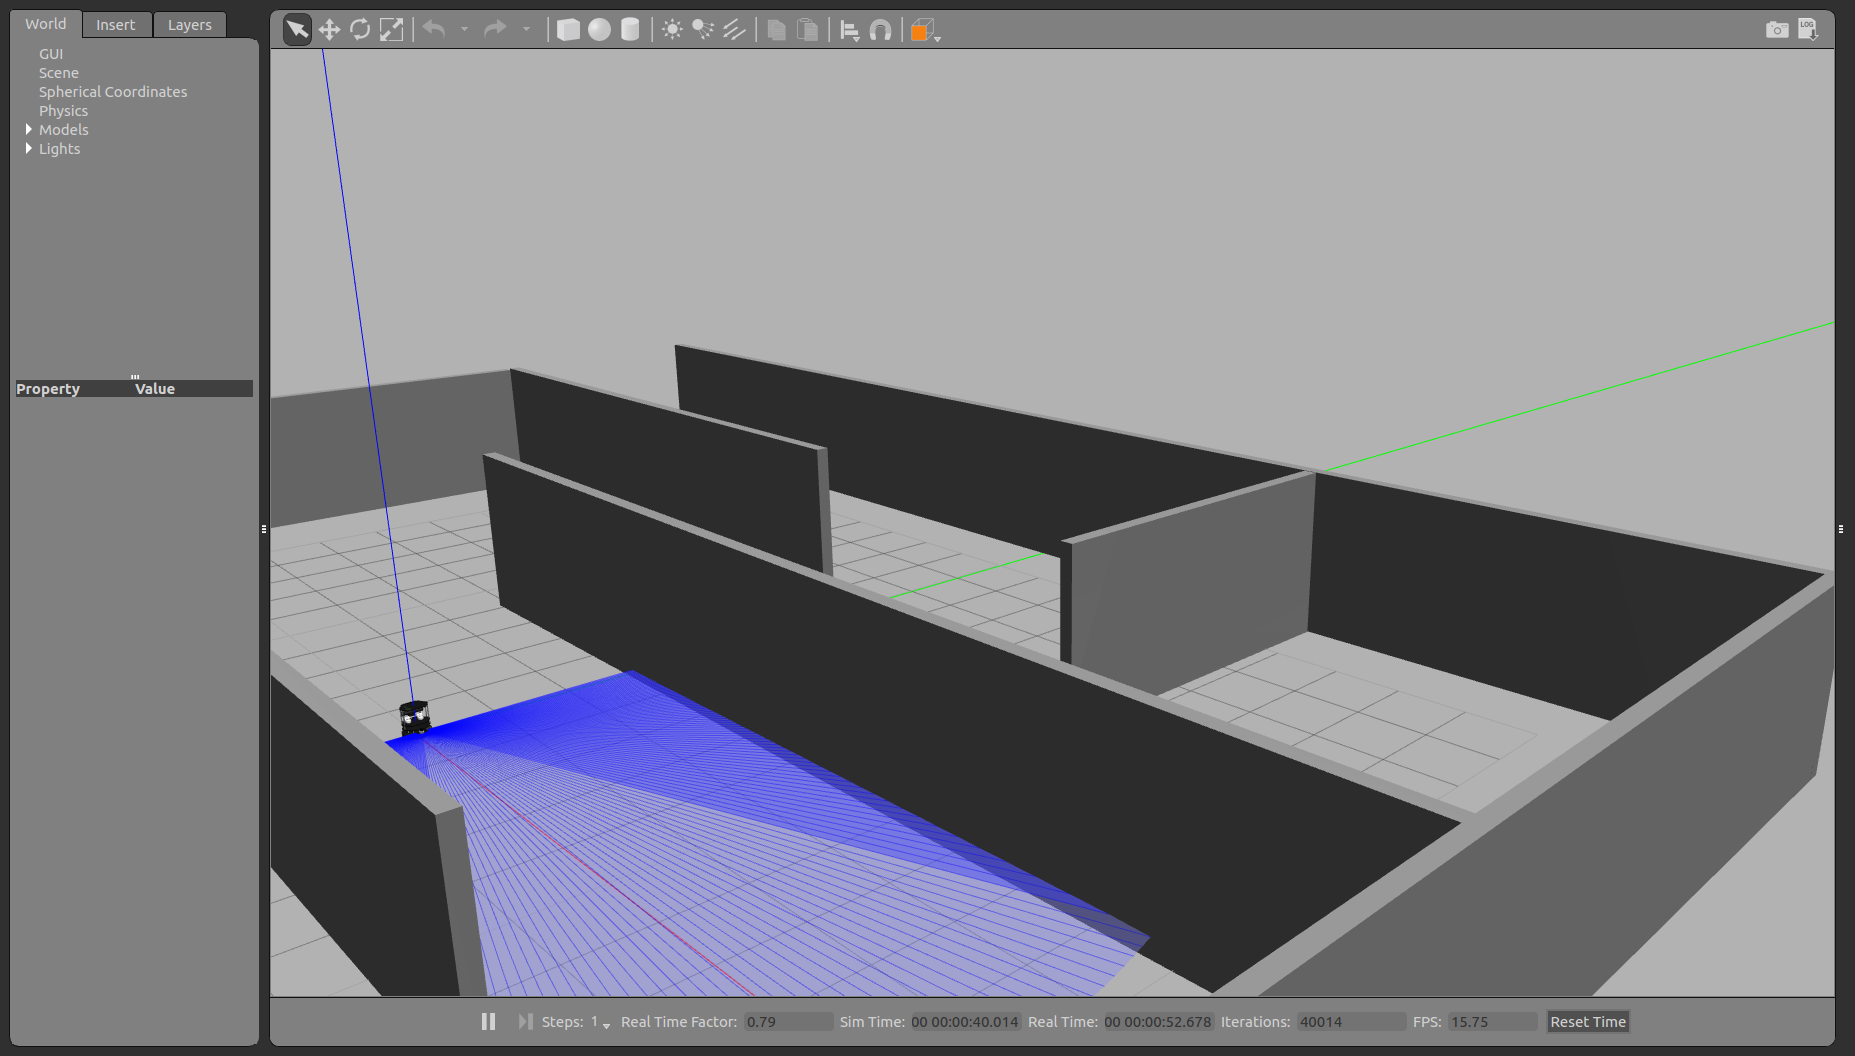
\includegraphics[width=0.8\textwidth]{figures/gazeboturtle.png}
    		\caption{Simulación del robot turtlebot con Gazebo}
		\label{fig.gazeboturtle}
		\end{center}
\end{figure}
\begin{figure}[H]
  \begin{center}
    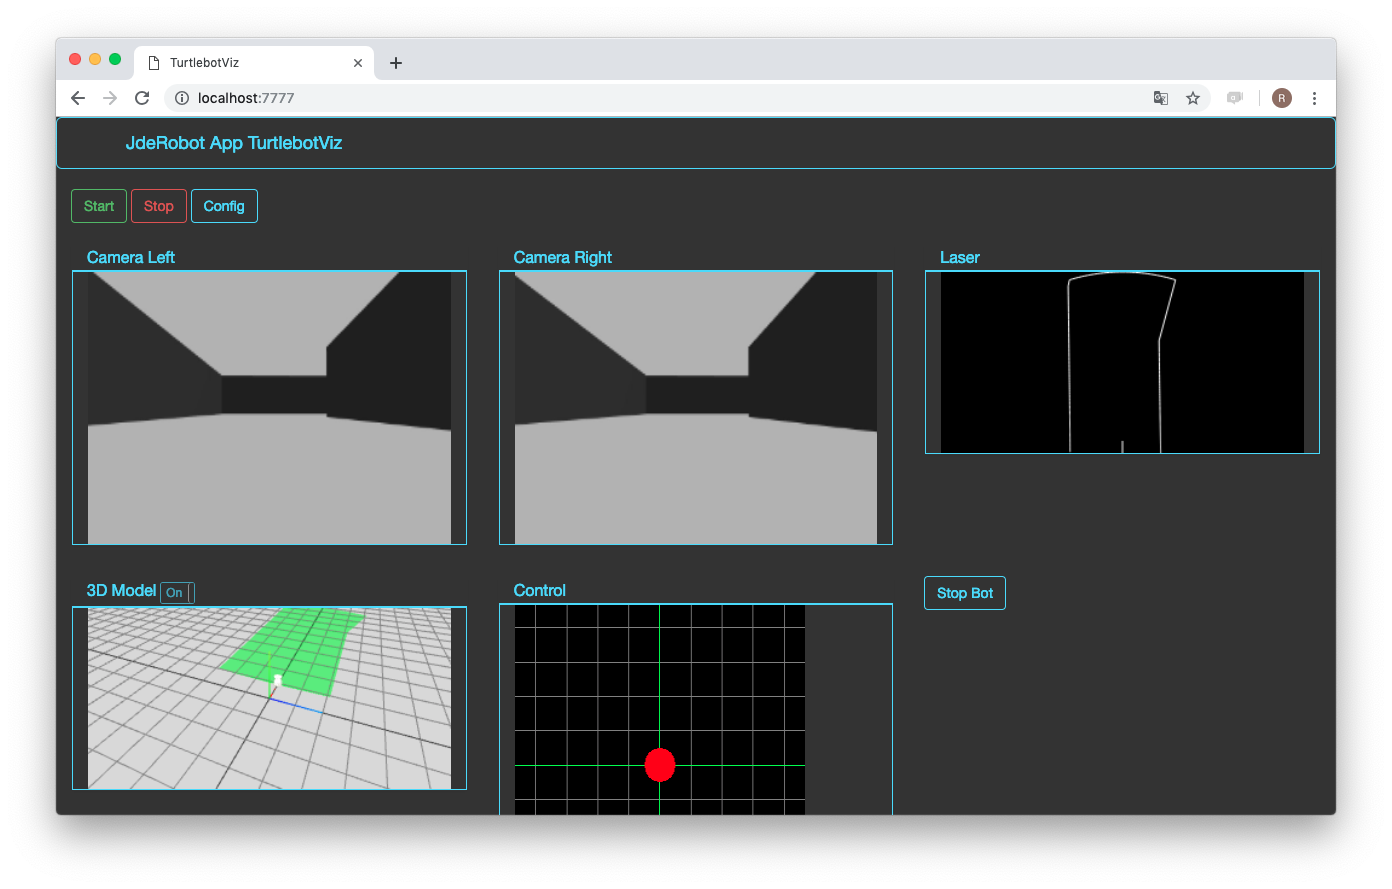
\includegraphics[width=0.8\textwidth]{figures/turtlebotviznode.png}
    		\caption{TurtlebotVizWeb ejecutado en un navegador web}
		\label{fig.turtlebotviznode}
		\end{center}
\end{figure}
\begin{figure}[H]
  \begin{center}
    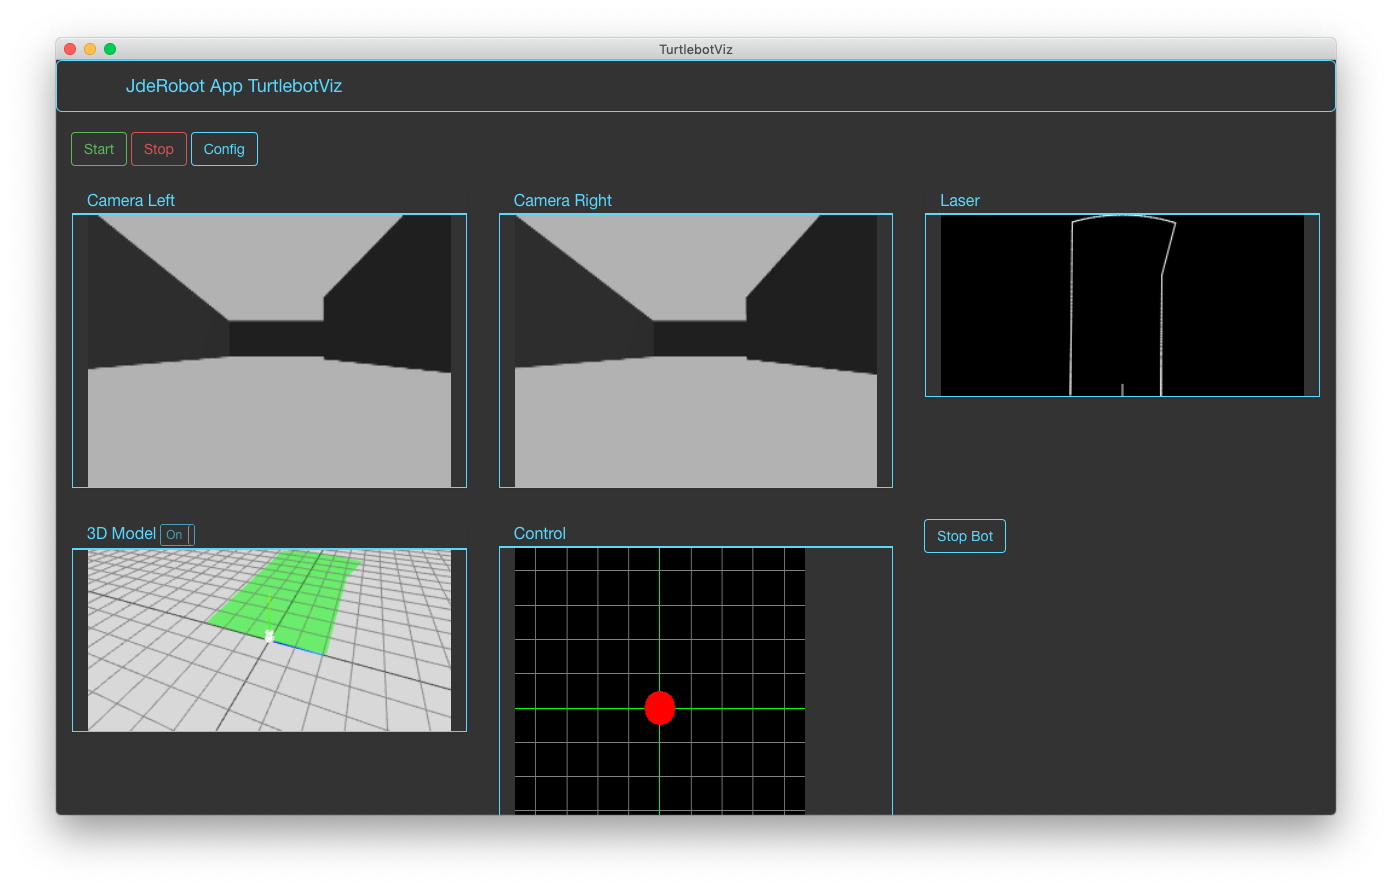
\includegraphics[width=0.8\textwidth]{figures/turtlebotvizelectron.png}
    		\caption{TurtlebotVizWeb ejecutado en Electron}
		\label{fig.turtlebotvizelectron}
		\end{center}
\end{figure}

\section{DroneVizWeb}
Se trata de un visor y teleoperador para Drones desarrollado con tecnologías web, que usa los middleware de comunicación ICE y ROS y pude ser ejecutados con Electron o en un navegador web.

\subsection{Diseño}
Al igual que en los visores anteriores, la versión previa de esta herramienta solo contaba con ICE como \textit{middleware} de comunicación. Ahora es capaz también de conectarse con Drones que se comuniquen mediante ROS y no solo mediante ICE. Para lograr la conectividad con el drone mediante ROS, ha sido necesaria la utilización de MavROS\footnote{\url{http://wiki.ros.org/mavros}} que es un paquete que proporciona una interfaz para el control de dones utilizando el protocolo MAVLink\footnote{\url{https://mavlink.io/en/}}. La figura 4.22 muestra el diagrama de bloques previo del sistema y la figura 4.23 muestra el diagrama tras la mejora realizada en este trabajo.

\begin{figure}[H]
  \begin{center}
    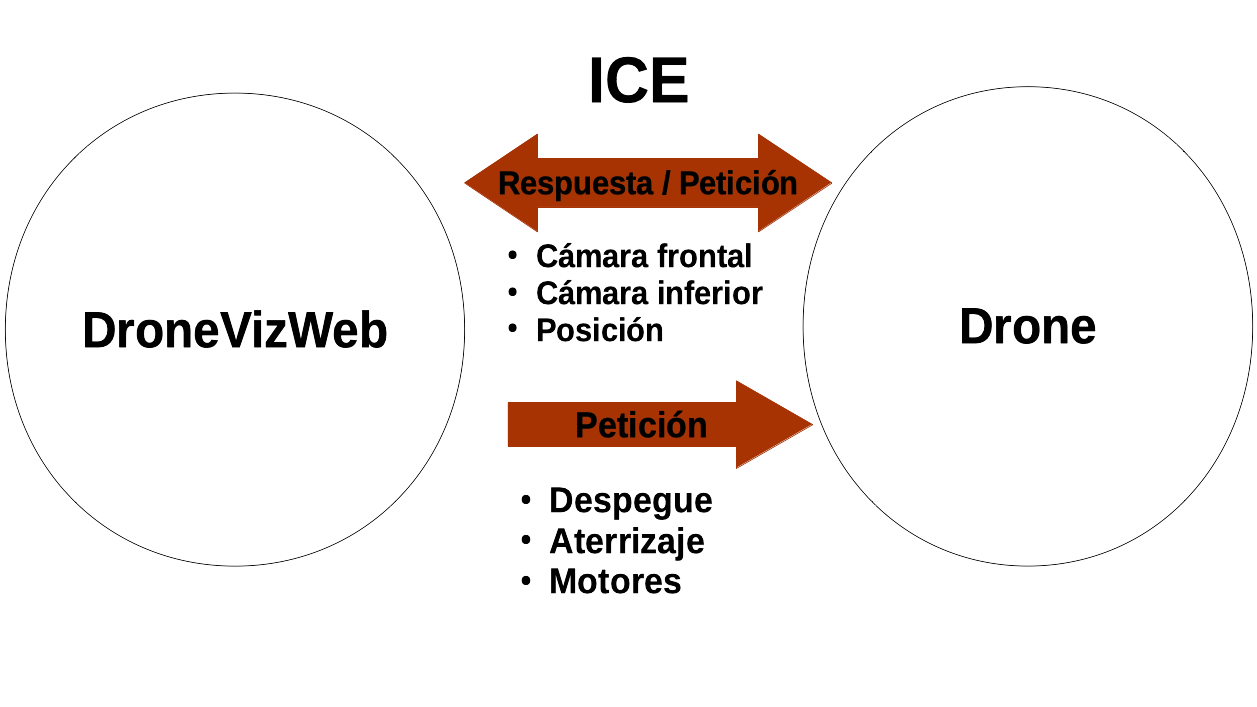
\includegraphics[width=0.8\textwidth]{figures/DroneViz1.png}
		\caption{Diagrama de bloques previo del sistema}
		\label{fig.esquematurtlebot1}
		\end{center}
\end{figure}

\begin{figure}[H]
  \begin{center}
    \includegraphics[width=0.8\textwidth]{figures/DroneViz2.png}
		\caption{Diagrama de bloques actual del sistema}
		\label{fig.esquematurtlebot2}
		\end{center}
\end{figure}

En la figura 4.24 muestra la estructura de la aplicación previa de una manera más detallada, mientras que la figura 4.25 muestra la estructura tras realizar la modificación.

\begin{figure}[H]
  \begin{center}
    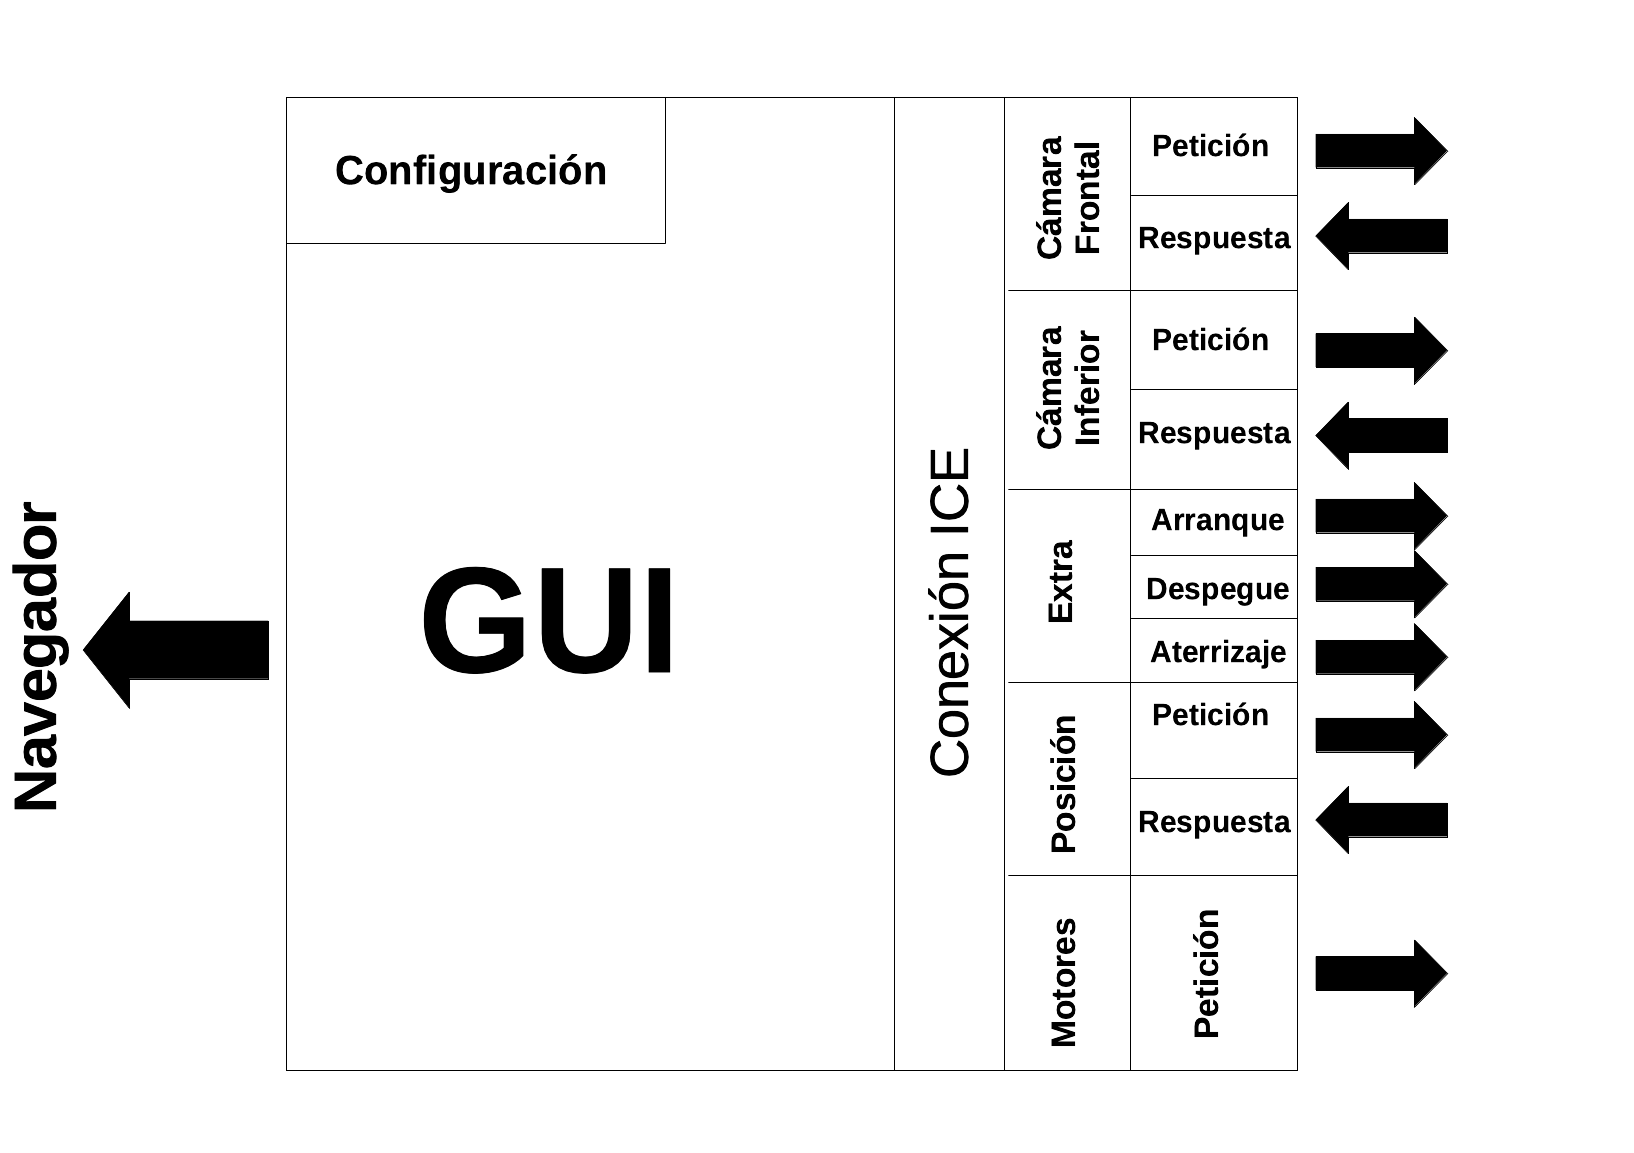
\includegraphics[width=0.8\textwidth]{figures/estrucuturadroneviz1.png}
		\caption{Estructura previa de la herramienta}
		\label{fig.estructuracamviz2}
		\end{center}
\end{figure}

\begin{figure}[H]
  \begin{center}
    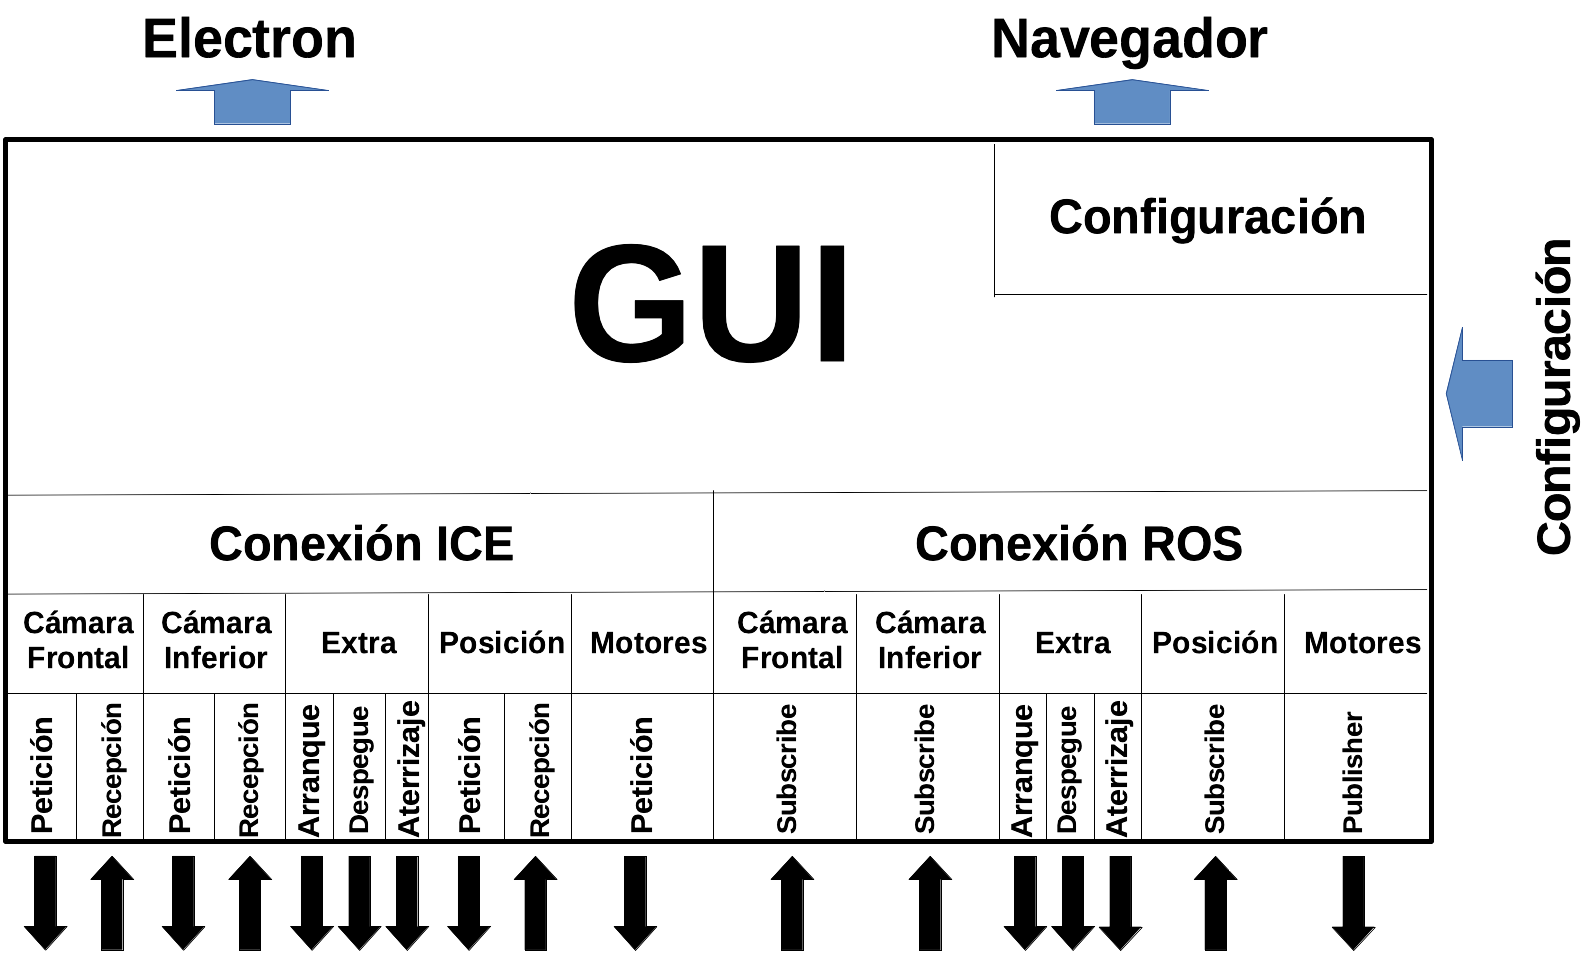
\includegraphics[width=0.8\textwidth]{figures/estrucuturadroneviz2.png}
		\caption{Estructura actual de la herramienta}
		\label{fig.estructuracamviz2}
		\end{center}
\end{figure}

Al igual que en las herramientas anteriores, esta dividida en dos partes: la interfaz gráfica y las conexiones. La interfaz gráfica contiene los elementos necesarios para visualizar los datos recibidos y teleoperar el drone, además de contener un menu para realizar la configuración en tiempo de ejecución del visor.

Para realizar las conexiones se utiliza los middleware de comunicación ROS y ICE. La versión de ICE como se ha indicado anteriormente es la existente de manera previa por lo que no es objeto de este trabajo profundizar en su funcionamiento. Únicamente indicar los mensajes que se transmiten ya que son los mismos que se transmiten usando ROS. El visor recibe dos mensajes simultáneamente procedente del drone, la imagen de la cámara (ya sea la cámara frontal o inferior) y la posición del drone. El visor envía la información sobre el control de los motores y las peticiones de arranque, despegue y aterrizaje del drone a la que se llama ``Extra'' ya que se realiza mediante la misma conexión.

En el caso de ROS, se utiliza los \textit{subscribe} para recibir los mensajes procedentes del robot, los \textit{publisher} para transmitir la información de los motores y los servicios de ROS para solicitar el arranque, despegue y aterrizaje al drone.

Por otro lado, al igual que para el resto de herramientas que componen este trabajo, se le añade la posibilidad de ejecutarse mediante el entorno Electron y la configuración previa mediante un archivo externo en formato ``YAML''.

\subsection{Interfaz gráfica}

La interfaz gráfica se mantiene la existente en la versión anterior de la herramienta. Esta interfaz cuenta con un elemento \texttt{Canvas} de HTML5 donde se muestra la imagen procedente de la cámara, sobre este elemento se incorporan tres botones, el primero botón es el utilizado para indicar el deseo de arrancar y despegar, el segundo botón es el que se utiliza para indicar el aterrizaje y el ultimo botón se utiliza para solicitar el cambio de cámara a mostrar (si en ese momento se muestra la cámara frontal, se cambia a la inferior y viceversa). Por otro lado, dentro de este elemento también se incorporan dos \textit{joysticks} para controlar el drone, estos \textit{joysticks} están creados usando también elementos \texttt{Canvas}, siendo el \textit{joystick} izquierdo el que controla la velocidad y el derecho el que controla la altura del drone. La interfaz gráfica cuenta con otro elemento \texttt{Canvas} donde se muestra la representación tridimensional del drone y su movimiento, así como tres botones para comenzar la conexión, para parar la conexión y para abrir la ventana con el menú para realizar la configuración en tiempo de ejecución. En la figura 4.26 se muestra la interfaz gráfica utilizada.

\begin{figure}[H]
  \begin{center}
    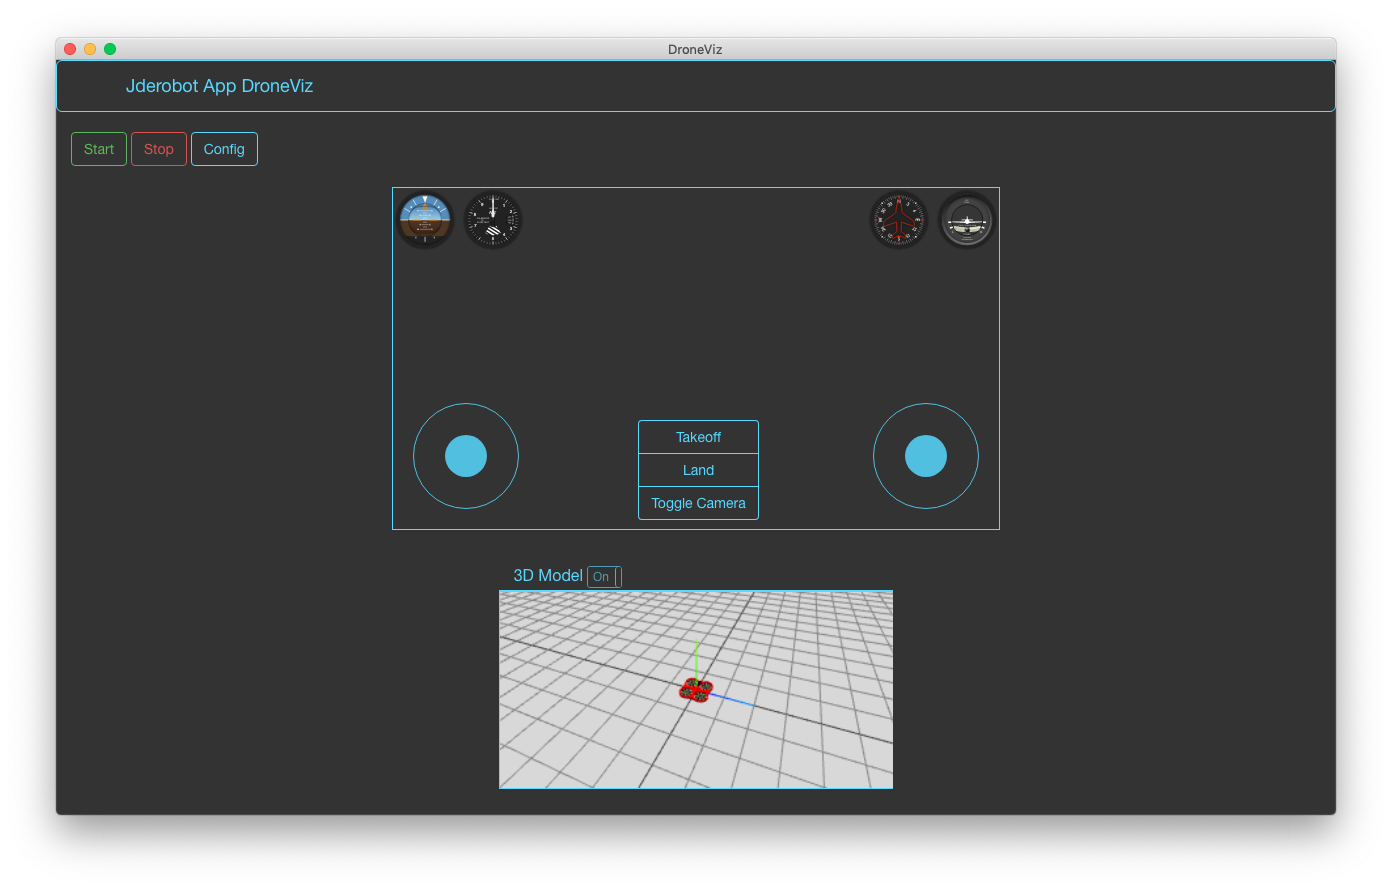
\includegraphics[width=0.8\textwidth]{figures/interfazdroneviz.png}
		\caption{Interfaz gráfica de DroneVizWeb}
		\label{fig.iterfazdroneviz}
		\end{center}
\end{figure}

Para poder configurar la conexión mediante ROS, se vuelve a utilizar lo indicado en la sección 4.2.2. En la figura 4.27 se muestra el menú de configuración para realizar la configuración en tiempo de ejecución.

\begin{figure}[H]
  \begin{center}
    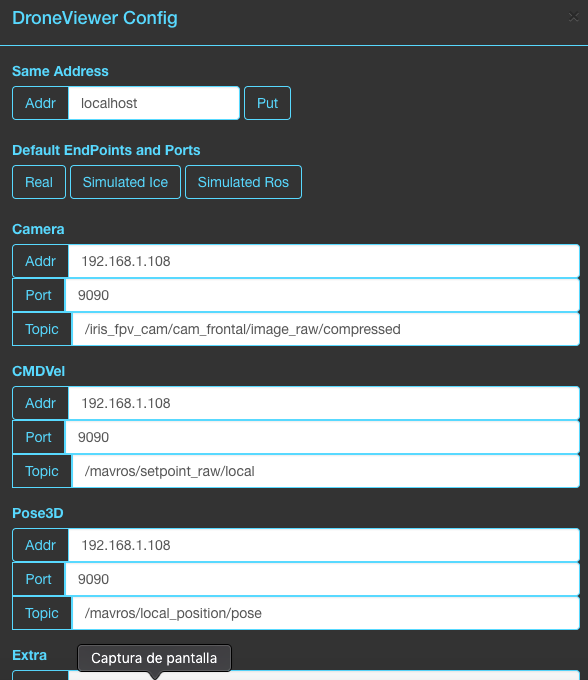
\includegraphics[width=0.8\textwidth]{figures/configdroneviz.png}
		\caption{Menu de configuración de DroneVizWeb}
		\label{fig.configdroneviz}
		\end{center}
\end{figure}

\subsection{Conexiones}

Con la modificación realizada la herramienta permite el uso de los middleware ICE y ROS para realizar las comunicaciones con un funcionamiento igual de eficiente.

Al igual que en el visor TurtlebotVizWeb, se reutilza el \textit{API} de ICE para definir los métodos y objetos necesarios para realizar la conexión mediante ROS.

\subsubsection{Establecimiento de las conexiones}

Por cada tipo de mensaje que se envía o se recibe se realiza una conexión, en el caso de este visor simultáneamente se tendrán activas 4 conexiones (cámaras, posición, motores y extra) como se ha podido ver en la figura 4.22 de la sección 4.3.1.

Dado que se establece la conexión de la misma forma que la explicada en la sección 4.2.3.1, no se va a profundizar más al respecto, simplemente indicar que los objetos creados en la \texttt{API} para realizar las conexiones en esta ocasión son \texttt{API.CameraRos, API.MotorsRos, API.ExtraRos y API.Pose3DRos} que corresponden con la conexión para la cámara, para el control de los motores, para el arranque, despegue y aterrizaje, y para la posición del drone respectivamente, con el método \texttt{connect} asociado a cada objeto y explicado en la sección anteriormente referenciada.

\subsubsection{Estructura de los mensajes}

Para este visor se van a utilizar los mensajes predeterminados de ROS para obtener las imágenes de la cámara y obtener la posición. Por otro lado, para transmitir las peticiones de arranque, despegue, aterrizaje y el control de los motores se utilizan los mensajes facilitados en el paquete MavROS\footnote{\url{http://docs.ros.org/melodic/api/mavros_msgs/html/index-msg.html}}. Para definir los mensajes se va a utilizar los mismos métodos que se usan en las herramientas anteriores.

El mensaje que transmite las imágenes de las cámaras son del tipo \texttt{sensor\_msgs/CompressedImage} y se define con el código que se muestra en el cuadro 4.29. Esta definición esta incluida dentro del método \texttt{connect} del objeto \texttt{API.CameraRos}.

\begin{lstlisting}[caption= Definición del mensaje para la información de las cámaras, label=cod.mensajecamdrone]
self.roscam = new ROSLIB.Topic({
            ros : self.ros,
            name : config.topic,
            messageType : "sensor_msgs/CompressedImage"
});
\end{lstlisting}

La información sobre el posicionamiento del drone se transmite mediante \texttt{nav\_msgs/Odometry}, que como se explicó en la sección 4.2.3.2, transmite la posición mediante la clase ``Pose3D''. En el cuadro 4.30 se muestra la definición de este mensaje que forma parte del método \texttt{connect} del objeto \texttt{API.Pose3DRos}

\begin{lstlisting}[caption= Definición del mensaje para obtener el posicionamiento del drone, label=cod.mensajeposedrone]
self.rospose = new ROSLIB.Topic({
		ros : self.ros,
		name : config.topic,
		messageType : "nav_msgs/Odometry"
});
\end{lstlisting}

La transmisión del control de los motores se envía mediante el tipo facilitado en el paquete MavROS \texttt{mavros\_msgs/PositionTarget}. Este mensaje transmite la información acerca de la posición para la coordenada ``x'', ``y'' y ``z'', la velocidad lineal en cada una de estos ejes de coordenadas, la aceleración en cada eje y la rotación entorno al eje ``y''. Con este mensaje se puede enviar toda la información para teleoperar un drone, además este mensaje incluye una marca de tiempo para sincronizar el drone con el teleoperador. Como en los casos anteriores, esta definición se incluye en el método \texttt{connect} del objeto \texttt{API.MotorsRos} y se puede ver en el cuadro 4.31.

\begin{lstlisting}[caption= Definición del mensaje para controlar los motores del drone, label=cod.mensajemotordrone]
self.rosMotors = new ROSLIB.Topic({
	ros : self.ros,
	name : config.topic,
	messageType : "mavros_msgs/PositionTarget"
});
\end{lstlisting}

Finalmente, los mensajes parta solicitar el arranque, despegue y aterrizaje se definen en el método \texttt{connect} del objeto \texttt{API.ExtraRos} y se muestran en el cuadro 4.32. El arranque se transmite mediante el mensaje del tipo \texttt{mavros\_msgs/CommandBool}, que envía únicamente un \textit{booleano} siendo el valor \textit{True} el que indica que arranque y \textit{False} el que indica que se apague el drone. Por otro lado, para el despegue y aterrizaje se utiliza el mismo tipo de mensaje contenido en el paquete de MavROS que es \texttt{mavros\_msgs/CommandTOL}. En este mensaje se envía información sobre la latitud, longitud, altitud y la rotación sobre el eje ``y''.

\begin{lstlisting}[caption= {Definición de los mensajes para arrancar, despegar y aterrizar}, label=cod.mensajeextradrone]
self.rosArming = new ROSLIB.Service({
	ros : self.ros,
	name : config.topic_arming,
	messageType : "mavros_msgs/CommandBool"
 });

self.rosTakeoff = new ROSLIB.Service({
	ros : self.ros,
	name : config.topic_takeoff,
	messageType : "mavros_msgs/CommandTOL"
});

self.rosLand = new ROSLIB.Service({
	ros : self.ros,
	name : config.topic_land,
	messageType : "mavros_msgs/CommandTOL"
});
\end{lstlisting}

\subsubsection{Subscripción a los \textit{Topic} y tratamiento de la información}

Mediante los \textit{subscribe} de ROS se obtienen las imágenes de las cámaras, así como la odometría del drone en cada momento. Para ello, los objetos \texttt{API.CameraRos} y \texttt{API.Pose3DRos} cuentan con el método \texttt{startStreaming}, sobre el cual se realiza la subscripción al \textit{topic} y se tratan los mensajes recibidos. Dado que el funcionamiento es el mismo que el explicado en la sección 4.1.3.3 para el caso de las cámaras y en la sección 4.2.3.3.3 para la información odometrica, no se profundiza de nuevo en esta sección.

En la figura 4.28 se puede ver la representación del drone que se muestra en el visor.

\begin{figure}[H]
  \begin{center}
    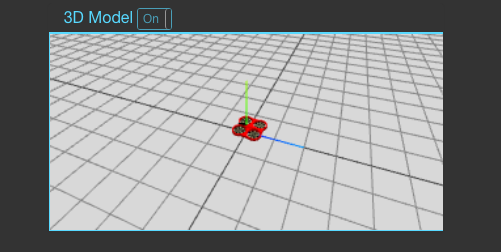
\includegraphics[width=0.8\textwidth]{figures/3ddrone.png}
		\caption{Representación 3D del drone}
		\label{fig.3ddrone}
		\end{center}
\end{figure}

\subsubsection{Publicación del mensaje con la información del teleoperador}

Para enviar la información acerca del control de los motores del drone, se utilizan los \textit{publisher} de ROS. Lo primero que hay que destacar es que los motores se controlan mediante dos \textit{joysticks} que se proyectan sobre el elemento \texttt{canvas} donde se muestra la imagen recibida por la cámara, tal y como se ha indicado en la sección 4.3.2. El \textit{joystick} izquierdo maneja la velocidad lineal (adelante, atrás, izquierda y derecha), mientras que con el \textit{joystick} derecho se indica la altura del drone.

Una vez se ha indicado esto, los siguiente es crear el mensaje con la información de los motores y publicarlo, para ello se ha definido el método \texttt{setMotors} dentro del objeto \texttt{API.MotorsRos} y que se muestra en el cuadro 4.33. Como se ha indicado en la sección 4.3.3.2, se va a utilizar el mensaje del tipo \texttt{mavros\_msgs/PositionTarget} proporcionado en el paquete MavROS.

\begin{lstlisting}[caption= Publicar el mensaje con la información del teleoperador, label=cod.publishetmotors]
self.setMotors = function(vel){
	var msg = {};
	var currentTime = new Date().getTime()-timestamp;
	var secs = Math.floor(currentTime/1000);
	var nsecs = Math.round(1000000000*(currentTime/1000-secs));
	msg.header = {};
	msg.header.stamp = {};
	msg.header.stamp.secs = secs;
	msg.header.stamp.nsecs = nsecs;
	msg.header.frame_id = "";
	msg.coordinate_frame = 8;
	msg.type_mask = 1475;
	msg.position = {};
	msg.position.x = 0;
	msg.position.y = 0;
	msg.position.z = vel.linearZ;
	msg.velocity = {};
	msg.velocity.x = vel.linearY;
	msg.velocity.y = vel.linearX;
	msg.velocity.z = 0;
	msg.acceleration_or_force = {};
	msg.acceleration_or_force.x = 0;
	msg.acceleration_or_force.y = 0;
	msg.acceleration_or_force.z = 0;
	msg.yaw = 0;
	msg.yaw_rate = 0;
	var motorsMessage = new ROSLIB.Message({
		header: msg.header,
		coordinate_frame: 8,
		type_mask: 1475,
		position: msg.position,
		velocity: msg.velocity,
		acceleration_or_force: msg.acceleration_or_force,
		yaw: 0,
		yaw_rate: 0
	});
	self.rosMotors.publish(motorsMessage);
}
\end{lstlisting}

Sobre el código del cuadro 4.34 lo primero que hay que indicar es que la información del teleoperador se le introduce al método por parámetro. Dentro del método se crea la marca de tiempo para incorporarla a la cabecera del mensaje y se definen el resto de parámetros de la cabecera. Posteriormente se definen el resto de parámetros que forman parte del tipo de mensaje escogido, sin embargo para transmitir el control de los motores únicamente se utilizan los parámetros correspondientes a la velocidad en su componente ``x'' e ``y'' para transmitir la velocidad lineal, y la posición en su componente ``z'' para manejar la altura del drone. El resto de parámetros del mensaje no se utilizan por lo que se da el valor ``0''. Posteriormente se crea el mensaje que se va a transmitir mediante \texttt{new ROSLIB.Message} y se publica.

Con este método se transmite un mensaje, pero se desea estar publicando mensajes con la información del teleoperador de manera continua. Al igual que se explica en la sección 4.2.3.4, se va a utilizar el método de HTML \texttt{setInterval} como se muestra en el cuadro 4.34.

\begin{lstlisting}[caption= Publicación continua del mensaje con la información del teleoperador, label=cod.intervalMotors]
var cmdvelInterval = setInterval(function(){cmdvel.setMotors(cmdSend);},1);
\end{lstlisting}

En la figura 4.29 se muestra el visor de las cámaras y los \textit{joysticks} para controlar los motores.

\begin{figure}[H]
  \begin{center}
    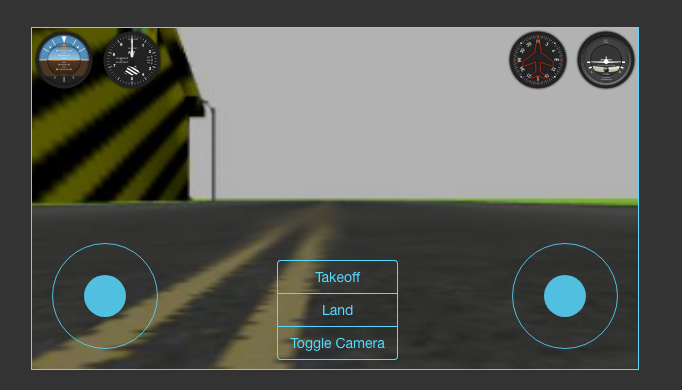
\includegraphics[width=0.8\textwidth]{figures/camaradrone.png}
		\caption{Visualización de las cámaras y control de los motores}
		\label{fig.camaradrone}
		\end{center}
\end{figure}

\subsubsection{Arranque, Despegue y Aterrizaje mediante Ros Services}

Para lograr arrancar, despegar y aterrizar el drone, es necesario usar los servicios de ROS proporcionados por el paquete MavROS. Estos servicios son complementarios entre si, es decir para despegar primero se ha debido arrancar los motores, para aterrizar ates se ha debido despegar y para apagar los motores antes se ha debido aterrizar. Teniendo en cuenta esto, es evidente que las llamadas a los métodos que realizan estas funciones deben realizarse de manera correlativa. Para lograr estos controles se han creado tres métodos dentro del objeto \texttt{API.ExtraRos} \texttt{Arming, takeoff y land}. Adicionalmente hay que remarcar la existencia de un cuarto método que es el encargado de cambiar el modo de pilotaje del drone y que de nuevo usa servicios de ROS, y se solicita una vez haya realizado el despegue del drone.

\begin{lstlisting}[caption= Método para arrancar o apagar los motores del drone, label=cod.arming]
self.arming = function(arranque){
	var request = new ROSLIB.ServiceRequest({
			value: arranque
	})
	self.rosArming.callService(request, function(result){
		if (arming){
			self.takeoff();
		} 
	});
}
\end{lstlisting}

En el código del cuadro 4.35 se muestra el método para realizar el arranque o apagado de los motores dependiendo lo que se envíe por parámetro al propio método. Si el valor del \textit{booleano} es verdadero, entonces se solicita el arranque mediante el servicio de ROS, si por el contrario es falos, se solicita su apagado. Para realizar la solicitud se utiliza el método de \texttt{roslibjs callService} y se le pasa por parámetro la petición creada mediante el objeto \texttt{new ROSLIB.ServiceRequest} y un manejador para el resultado. En caso de que el resultado sea positivo y se se solicite el arranque, se llama al método que realiza la solicitud de despegue, si se trata del apagado de los motores no se realiza nada, ya que el drone queda a la espera de una nueva solicitud de arranque.

\begin{lstlisting}[caption= Método para arrancar o apagar los motores del drone, label=cod.takeoff]
self.takeoff = function(){
	var request = new ROSLIB.ServiceRequest({
		altitude:5.5,
		latitude: 0,
		longitude: 0,
		min_pitch: 0,
		yaw: 0
	});
	self.rosTakeoff.callService(request, function(result) {
		console.log("TakeOff Done");
		self.setmode();
	});
}
\end{lstlisting}

En el cuadro 4.36 se muestra el método para realizar el despegue. En la petición de despegue se debe enviar información acerca de la latitud, longitud, altitud, orientación entorno al eje ``y'' y el ángulo de vision. Dado que solo interesa indicar la altura, se dejan todos los valores a ``0'', menos la altitud que se fija un valor de ``5.5''. Posteriormente se vuelve a enviar la solicitud del mismo modo que para el arranque o apagado. En caso de que el resultado sea positivo, se llama al método para cambiar el modo de pilotaje del drone.

\begin{lstlisting}[caption= Método para cambiar el modo de pilotaje, label=cod.setMode]
self.setmode = function(){
	var request = new ROSLIB.ServiceRequest({
		custom_mode: "OFFBOARD"
	});
	self.rosSet_Mode.callService(request, function(result){
	})
}
\end{lstlisting}

En el cuadro 4.37 se muestra el método para cambiar el modo de pilotaje del drone. Una vez el drone ha despegado se le solicita que cambie el modo de piloto automático por el modo ``OFFBOARD'', de modo que se puedan controlar los motores mediante el teleoperador del visor. En este caso, una vez el resultado de la solicitud es afirmativo, no se realiza ninguna nueva acción al estar listo el drone ya listo para ser pilotado, por tanto el drone queda a la espera de la información con el control de los motores o la petición de aterrizaje.

\begin{lstlisting}[caption= Método para cambiar el modo de pilotaje, label=cod.setMode]
this.land = function(){
	var request = new ROSLIB.ServiceRequest({
		min_pitch: 0,
		yaw: 0,
		latitude: 0,
		longitude: 0,
		altitude:0,
	});
	self.rosLand.callService(request, function(result){
		self.arming(false);
	})
}
\end{lstlisting}

El cuadro 4.38 contiene el código del método que realiza la solicitud de aterrizaje. Se puede apreciar que la petición es igual a la realizada para indicar el despegue, salvo que la altitud que se envía ahora es ``0'' y no ``5.5'' como en el despegue. Una vez que se envía la solicitud de aterrizaje y el resultado es positivo, se llama al método del cuadro 4.35 pasando por parámetro el \textit{booleano false} para indicar que se solicita el apagado de los motores.

\subsection{Configuración}
Al igual que los dos visores anteriores, se puede realizar la configuración mediante la utilización de un archivo del tipo ``YAML'', tratando el archivo de la misma forma que se explica en la sección 4.1.4,  o a través de la configuración en tiempo de ejecución mediante el menu de configuración de la interfaz gráfica que se explica en la sección 4.3.2.

Los parámetros configurables para este visor son los siguientes:
\begin{itemize}
\item \textit{Middleware} utilizado para realizar la comunicación. Por defecto es Ros.
\item Dirección IP para conectar el visor a la cámara frontal del drone. Por defecto ``localhost''.
\item Puerto para conectar el visor a la cámara frontal del drone. Por defecto es ``9090''.
\item Endpoint para conectar el visor a la cámara frontal del drone (en caso de ROS será el topic utilizado para realizar esta conexión). Por defecto es ``/iris\_fpv\_cam/cam\_frontal/image\_raw/compressed''
\item Dirección IP para conectar el visor a la cámara inferior del drone. Por defecto ``localhost''.
\item Puerto para conectar el visor a la cámara inferior del drone. Por defecto es ``9090''.
\item Endpoint para conectar el visor a la cámara inferior del drone(en caso de ROS será el topic utilizado para realizar esta conexión). Por defecto es ``/iris\_fpv\_cam/cam\_ventral/image\_raw/compressed''
\item Dirección IP para conectar el visor a la odometría del drone. Por defecto ``localhost''.
\item Puerto para conectar el visor a la odometría del drone. Por defecto es ``9090''.
\item Endpoint para conectar el visor a la odometría del drone (en caso de ROS será el topic utilizado para realizar esta conexión). Por defecto es ``/mavros/local\_position/pose''
\item Dirección IP para conectar el visor a los extras (arranque, despegue, etc) del drone. Por defecto ``localhost''.
\item Puerto para conectar el visor  a los extras (arranque, despegue, etc) del drone. Por defecto es ``9090''.
\item Endpoint para conectar el visor  a los extras (arranque, despegue, etc) del drone (en caso de ROS será el topic utilizado para realizar esta conexión). Por defecto es ``ardrone\_extra''
\item Dirección IP para conectar el visor con los motores del drone. Por defecto ``localhost''.
\item Puerto para conectar el visor con los motores del drone. Por defecto es ``9090''.
\item Endpoint para conectar el visor con los motores del turtlebot (en caso de ROS será el topic utilizado para realizar esta conexión). Por defecto es ``/mavros/setpoint\_raw/local''
\end{itemize}

\subsubsection{Experimentos}
Al igual que todas la herramientas que forman este trabajo, este visor puede ser ejecutado mediante un navegador web o Electron. Para realizar los experimentos, se va a utilizar el simulador Gazebo en su versión de ROS\footnote{\url{http://wiki.ros.org/gazebo_ros}} junto con el drone PX4\footnote{\url{https://px4.io/}}.

En un primer terminal o consola se debe ejecutar el servidor intermedio de ROS que se puede ver en el esquema.
\begin{lstlisting}[caption= Ejecución del servidor intermedio, label=cod.servidorintermediodrone]
#>roslaunch rosbridge_server rosbridge_websocket.launch
\end{lstlisting}

En un segundo terminal se ejecuta gazebo con la simulación del drone PX4.

\begin{lstlisting}[caption= Ejecución de gazebo con el drone PX4 label=cod.gazebodrone]
#>roslaunch gazebo_ros follow\_road.launch
\end{lstlisting}

En el tercer terminal se ejecuta DroneVizWeb.

\begin{itemize}
\item Como aplicación web utilizando Node.js
\end{itemize}
\begin{lstlisting}[caption= Ejecución con Node.js, label=cod.dronenodejs]
#>node run.js
Se arranca el navegador y se introduce la URL http://localhost:7777/
\end{lstlisting}
\begin{itemize}
\item Como aplicación de escritorio con Electron
\end{itemize}
\begin{lstlisting}[caption= Ejecución con Electron, label=cod.droneelectron]
#>npm install
#>npm start
\end{lstlisting}

\begin{figure}[H]
  \begin{center}
    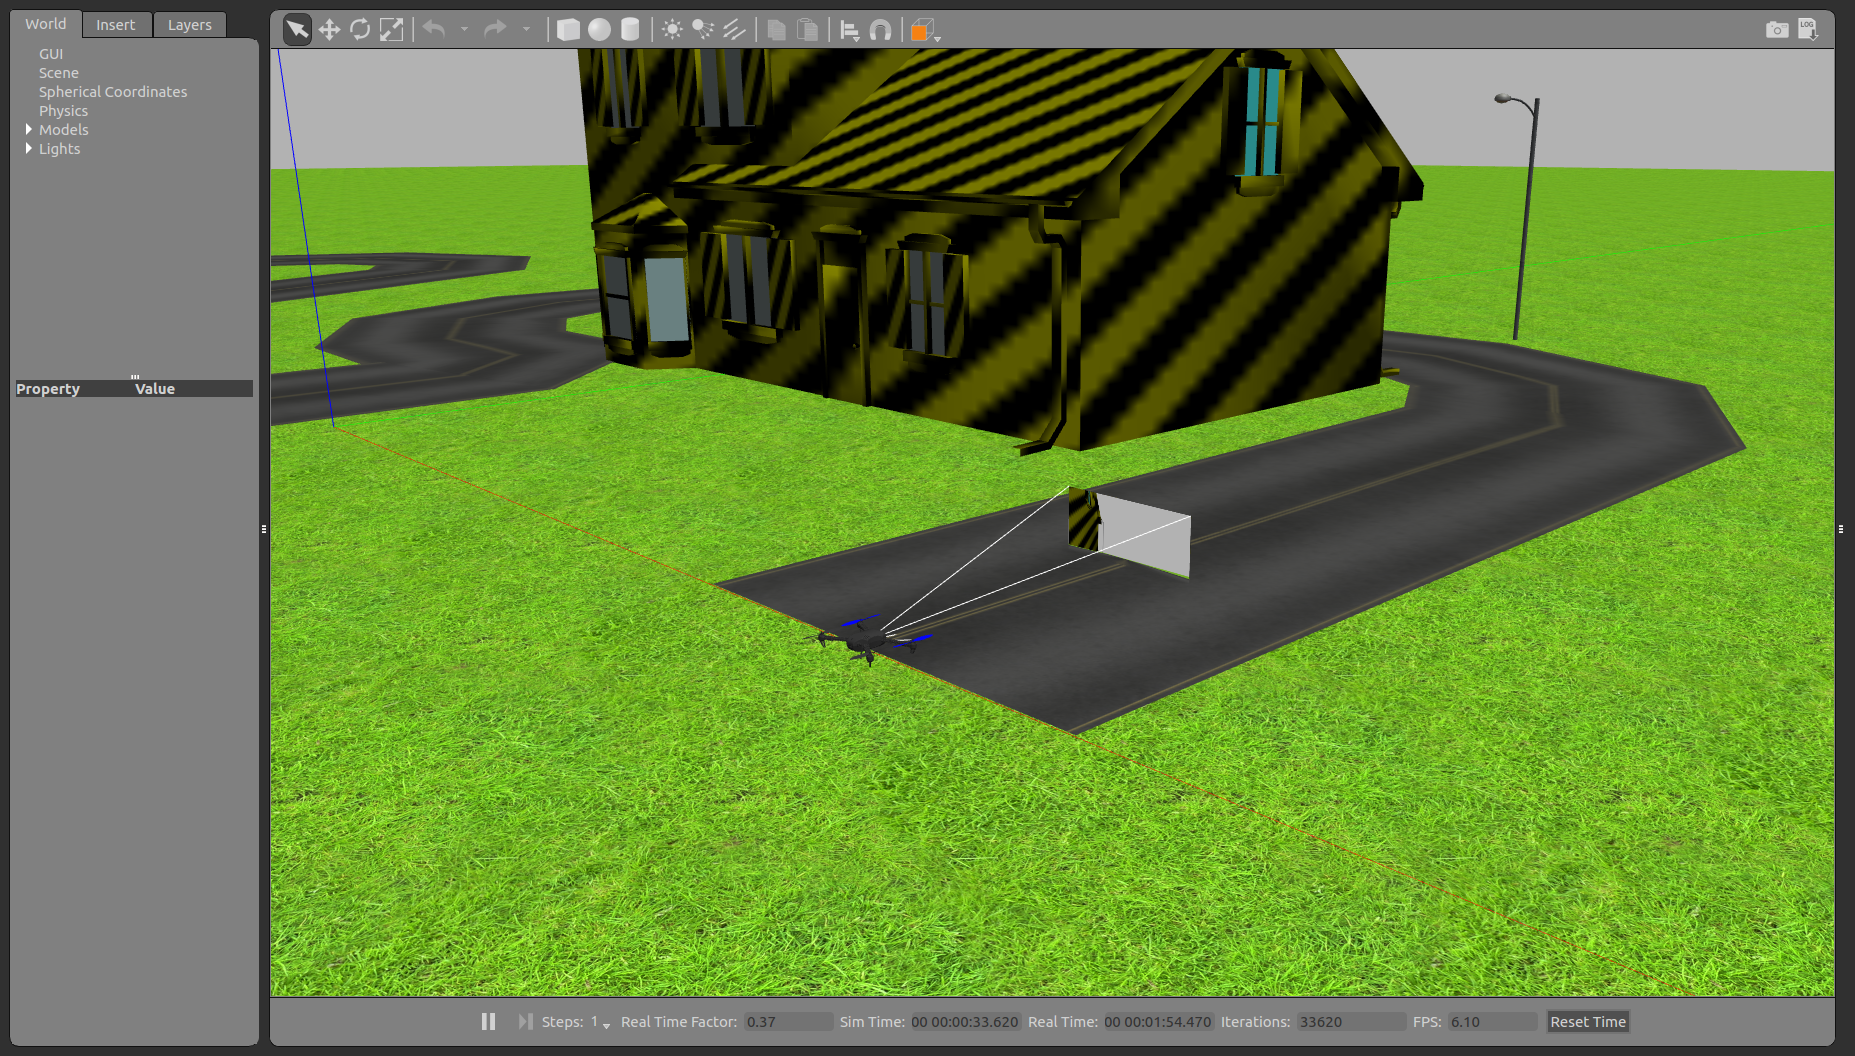
\includegraphics[width=0.8\textwidth]{figures/gazebodrone.png}
    		\caption{Simulación del drone con Gazebo}
		\label{fig.testcamserver1}
		\end{center}
\end{figure}
\begin{figure}[H]
  \begin{center}
    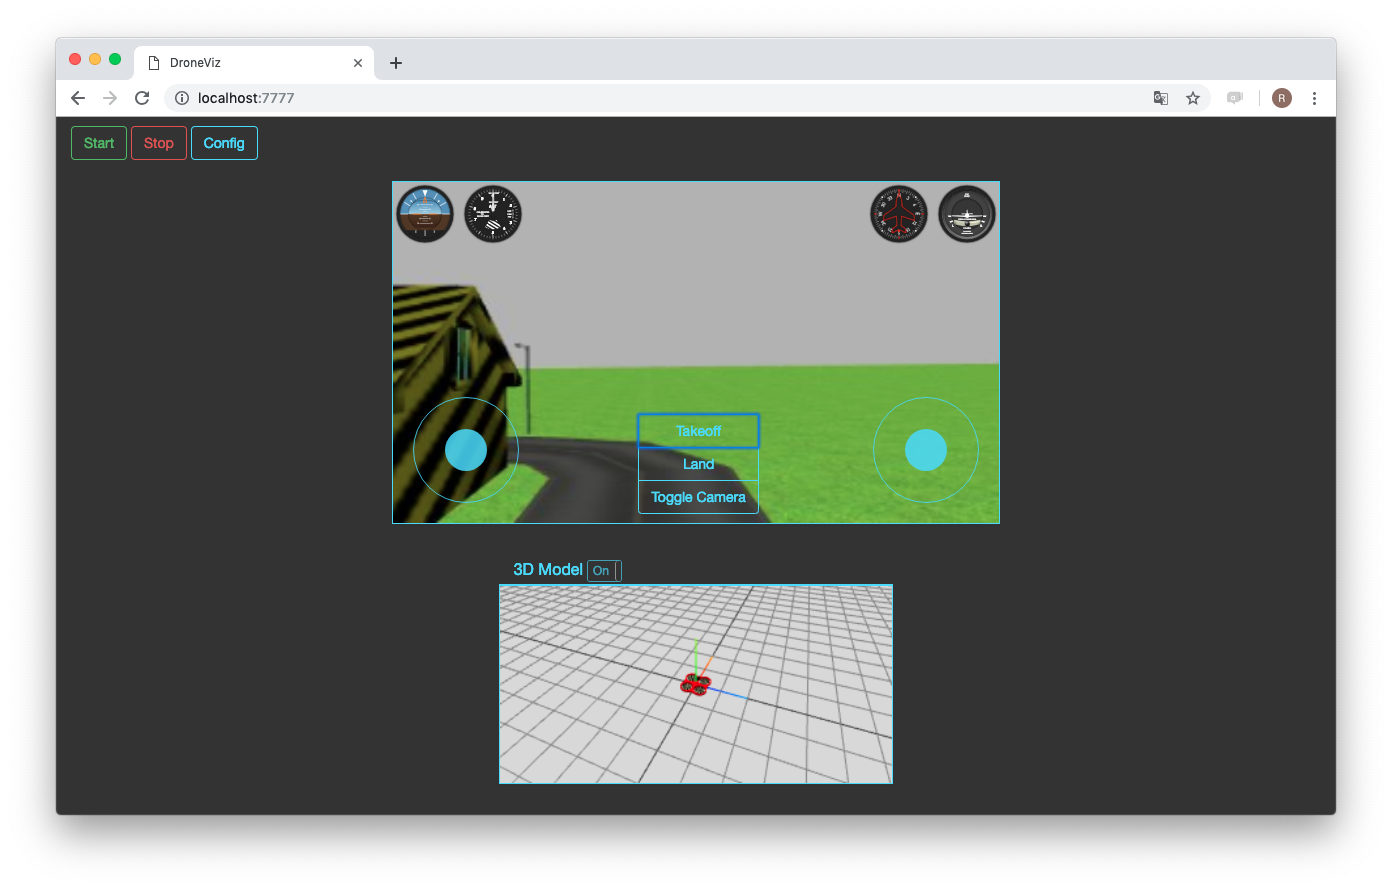
\includegraphics[width=0.8\textwidth]{figures/droneviznode.png}
    		\caption{DroneVizWeb ejecutado en un navegador web}
		\label{fig.droneviznode}
		\end{center}
\end{figure}
\begin{figure}[H]
  \begin{center}
    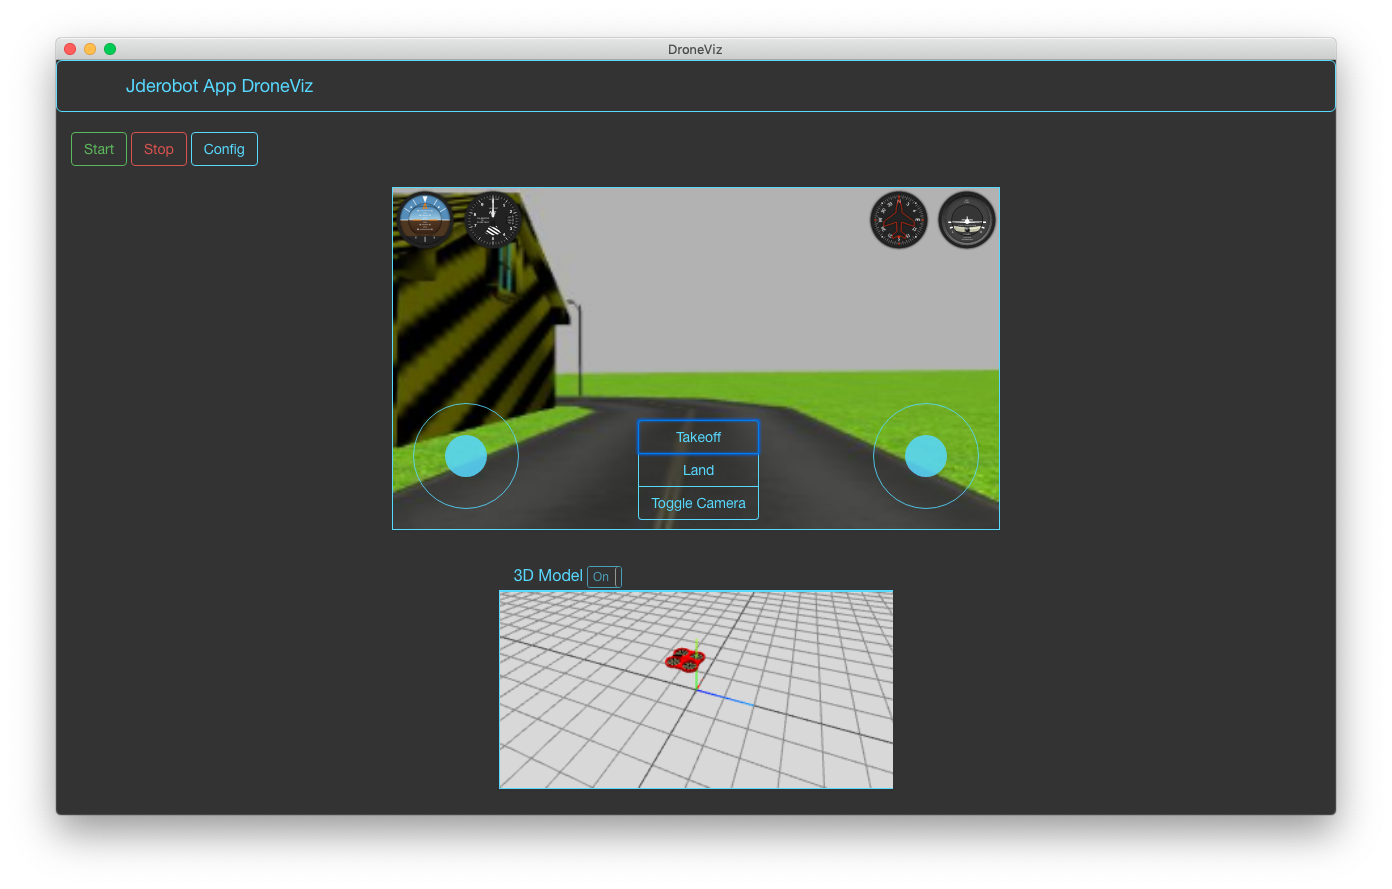
\includegraphics[width=0.8\textwidth]{figures/dronevizelectron.png}
    		\caption{DroneVizWeb ejecutado en Electron}
		\label{fig.dronevizelectron}
		\end{center}
\end{figure}










